\documentclass[a4paper,oneside]{book}
\usepackage{float}
\usepackage{amsmath}
\usepackage{xcolor}
\usepackage{lipsum}
\usepackage[hidelinks]{hyperref}
\usepackage[a4paper, total={7.27in, 10.69in}]{geometry}
\usepackage{titletoc}
\usepackage{graphicx}
\usepackage{tikz} % for drawing labeled lines
\usetikzlibrary{calc} % for drawing labeled lines

\titlecontents*{chapter}
  [0pt]% <left>
  {}
  {\chaptername\ \thecontentslabel\quad}
  {}
  {\bfseries\hfill\contentspage}    

\usepackage{bookmark}
\usepackage{etoolbox}

\makeatletter
\newcommand*{\AddChapterPrefixInBookmarks}{%
  \if@mainmatter
    \ifnum\bookmarkget{level}=0 %
      \preto\bookmark@text{\@chapapp\space}%
    \fi
  \fi
}
\makeatother

\bookmarksetup{
  numbered,
  addtohook=\AddChapterPrefixInBookmarks,
}

% Workaround for numbered sections in unnumbered
% chapter "Introduction" to avoid chapter number
% zero.
\renewcommand*{\thesection}{%
  \ifcase\value{chapter}%
  \else
    \thechapter.%
  \fi
  \arabic{section}%
}

\title{My document}
\pagestyle{headings}

\begin{document}
\frontmatter

\begin{titlepage}
    \begin{center}
        \vspace*{1cm}
            
        \Huge
        \textbf{Statistics Question Bank}
            
        \vspace{0.5cm}
        \LARGE
        First Paper
            
        \vspace{1.5cm}
            
        \textbf{Abdullah Al Mahmud}
            
        \vfill
            
            
        \vspace{0.8cm}
            
 \includegraphics[width=1cm]{logo}
 
        \Large
        www.statmania.info\\
            
    \end{center}
\end{titlepage}

\tableofcontents


\mainmatter

\chapter{Statistics, Variable and Concepts of Different Symbols} 

\section{Creative Questions}

\begin{enumerate}

     \item
	  \textbf{A system analyst collected frequencies of a signal at different times. Then he realized due to some unknown noise, 0.5 units got added to all the values. The recorded values are given below:} 
	  
	  \begin{center}
	  10, 12, 15, 14, 12, 16, 20, 16, 18, 11
	  \end{center}
  
  \begin{enumerate}
    \item
	What is change of origin? \hfill 1
    \item
	Does change of origin have an effect on median? \hfill 2
    \item  
	Find $\displaystyle \sum_{i=1}^{10} (X_i-5)$. \hfill 3
    \item
	Determine the summation of the values discarding the noise. \hfill 4
  \end{enumerate}
  
  \item  
\textbf{The daily website visits (in thousands) for an online platform over seven days are recorded as 80, 85, 90, 95, 100, 105, and 110 (denoted by \textit{z}). The platform analyst claimed that the square of the total visits is greater than the total of the squared visits.}

\begin{enumerate}
    \item  
    Calculate $\displaystyle \sum_{i=1}^7 (z_i - 2z_i)^2$ using the provided data. \hfill 3
    \item
    Verify whether the analyst’s statement is accurate based on the data. \hfill 4
\end{enumerate}
  
  \item
\textbf{A software developer tracked the response times (in milliseconds) 
of a web application under test during peak usage hours. An unexpected 
delay of 1.2 ms was added to each recorded response time due to server
lag. The recorded times are as follows:}

\begin{center}
45, 48, 52, 50, 47, 53, 60, 55, 58, 49
\end{center}

\begin{enumerate}
    \item  
    Calculate $\displaystyle \sum_{i=1}^{10} (X_i - 25)$. \hfill 3
    \item
    Find the sum of the original response times before the lag was added. \hfill 4
\end{enumerate}

  
  \item
\textbf{The monthly sales (in thousands of units) recorded by a store over 
five months are 120, 135, 150, 160, and 175. The store manager 
stated that the square of the total sales is greater than the total of 
the squared sales.}

\begin{enumerate}
    \item  
    Calculate $\displaystyle \sum_{i=1}^5 (x_i - 1.5x_i)^2$ using the 
    provided data. \hfill 3
    \item
    Assess whether the manager’s statement is accurate based on the data. \hfill 4
\end{enumerate}

  \item  
  \textbf{A nutritionist is analyzing the daily protein intake (in grams) of five athletes.  
  The recorded values are:}  
  \begin{center}
  $x_1 = 55,\quad x_2 = 60,\quad x_3 = 48,\quad x_4 = 62,\quad x_5 = 50$
  \end{center}

  \begin{enumerate}
    \item  
    Compute the value of $\displaystyle \sum_{i=1}^5 (x_i - 52)^2$. \hfill 3

    \item  
    Calculate $\displaystyle \sum_{i=1}^5 (x_i^2 - 4x_i + 10)$ using both direct evaluation and by separating the summation terms. \hfill 4
  \end{enumerate}

 \item
	  \textbf{Marks obtained by five students in statisics out of 15 were 4, 6, 10, 12, and 15. The examiner said, the square of the sum of the marks is greater than the sum of the squares of the marks.} 
  
  \begin{enumerate}
    \item
	What is finite population? \hfill 1
    \item
	Explain quantitative variable with an example. \hfill 2
    \item  
	In the light of the available data, find $\displaystyle \sum_{i=1}^5 (x_i-2x_i)^2$ \hfill 3
    \item
	Verify the comment of the examiner. \hfill 4
  \end{enumerate}
  
  \item
\textbf{The revenue and expenses (in million BDT) of different business sectors are shown below:}

\begin{table}[h]
\centering
\begin{tabular}{c|ccccc}
Sector & 1 & 2 & 3 & 4 & 5 \\ \hline
Revenue (X) & 45 & 32 & 50 & 60 & 40 \\ \hline
Expenses (Y) & 30 & 20 & 35 & 50 & 25
\end{tabular}
\end{table}

\begin{enumerate}
    \item  
    Find the value of $\displaystyle \sum_{i=1}^5 \sum_{j=1}^5 (x_i - y_j)$. \hfill 3
    \item
    Examine the statement theoretically and empirically:  $\displaystyle \sum_{i=1}^5 (3x_i - 4y_j) = 3 \sum_{i=1}^5 x_i - 4 \sum_{i=1}^5 y_j$. \hfill 4
\end{enumerate}


   \item
	  \textbf{The capital and profit (in million BDT) of some Bangladeshi 
	  industries are given below:}
	  
	  \begin{table}[h]
	  \centering
\begin{tabular}{c|ccccc}
Industry & 1 & 2 & 3 & 4 & 5 \\ \hline
Capital (X) & 20 & 15 & 26 & 31 & 18 \\ \hline
Profit (Y) & 15 & 10 & 17 & 25 & 10
\end{tabular}
\end{table}
  
  \begin{enumerate}
    \item
	What is finite population? \hfill 1
    \item
	What are the functions of statistics? \hfill 2
    \item  
	Find the value of $\displaystyle \sum_{i=1}^5 \sum_{j=1}^5 (x_i - y_j)$ \hfill 3
    \item
	Analyze the statement theoretically and empirically:  $\displaystyle \sum_{i=1}^5 (4x_i-6y_j) = 4 \sum_{i=1}^5 x_i - 6 \sum_{i=1}^5 y_j $ \hfill 4
  \end{enumerate}
  
  \item  
	  \textbf{The revenue and expenditure (in million BDT) of five companies in Bangladesh are given below:}  
	  
	  \begin{table}[h]
	  \centering
\begin{tabular}{c|ccccc}
Company & A & B & C & D & E \\ \hline
Revenue (X) & 50 & 40 & 60 & 55 & 45 \\ \hline
Expenditure (Y) & 30 & 25 & 35 & 40 & 28
\end{tabular}
\end{table}
  
  \begin{enumerate}
    \item  
	Compute $\displaystyle \sum_{i=1}^5 (x_i - y_i)$. Interpret the result in terms of net earnings. \hfill 3  
    \item  
	Show that $\displaystyle \sum_{i=1}^5 (3x_i - 2y_i) = 3 \sum_{i=1}^5 x_i - 2 \sum_{i=1}^5 y_i$ theoretically and empirically. \hfill 4  
  \end{enumerate}  

  
  \item
\textbf{The monthly sales and expenses (in thousand BDT) of five retail stores are given below:}

\begin{table}[h]
\centering
\begin{tabular}{c|ccccc}
Store & A & B & C & D & E \\ \hline
Sales (X) & 50 & 65 & 40 & 70 & 55 \\ \hline
Expenses (Y) & 30 & 45 & 25 & 50 & 35
\end{tabular}
\end{table}

\begin{enumerate}
    \item 
    Calculate $\displaystyle \sum_{i=1}^5 (x_i + y_i)$ \hfill 3
    \item 
    Verify whether the statement $\displaystyle \sum_{i=1}^5 (3x_i - 2y_i) = 3 \sum_{i=1}^5 x_i - 2 \sum_{i=1}^5 y_i$ holds true. \hfill 4
\end{enumerate}


\item
	  \textbf{Goals scored by a footballer in 25 matches are summarized as shown below.} 
	  
	  \begin{table}[h]
	  \centering
\begin{tabular}{|c|ccccc|}
Goals & 0 & 1 & 2 & 3 & 4 \\ \hline
Times & 8 & 9 & 5 & 2 & 1
\end{tabular}
\end{table}
  
  \begin{enumerate}
    \item
	Is no. goals a discrete or continuous variable? \hfill 1
    \item
	Verify theoretically: $\displaystyle \sum_{i=1}^{2} X_iY_i = \sum_{i=1}^{2} X_i \times \sum_{i=1}^{2} Y_i$ \hfill 2
    \item  
	Find the total number of goals using a suitable notation. \hfill 3
    \item
	If he scores two (2) goals in the next match, will the scoring rate increase? Explain logically and empirically \hfill 4
  \end{enumerate}
  
  \item
\textbf{Points scored by a basketball player in 20 games are summarized as shown below.}

\begin{table}[h]
\centering
\begin{tabular}{|c|ccccc|}
Points & 0 & 1 & 2 & 3 & 4 \\ \hline
Games  & 4 & 6 & 5 & 3 & 2
\end{tabular}
\end{table}

\begin{enumerate}
    \item  
    Find the total number of points scored using appropriate notation. \hfill 3
    \item
    If he scores five (5) points in the next game, will the average scoring rate increase? Justify your answer with calculations. \hfill 4
\end{enumerate}

  
    \item  
	  \textbf{A researcher conducting a study on economic indicators has gathered the following data points, representing the net income (in million BDT) of five different companies over a fiscal year:}  
	  
	  \begin{center}  
	  $x_1=15, x_2=-12, x_3=10, x_4=21, x_5=33$  
	  \end{center} 
  \begin{enumerate}
    \item
	What is sample? \hfill 1
    \item
	Briefly explain shift or origin and scale. \hfill 2
    \item  
	Compute the value of $\displaystyle \sum_{i=1}^5 (x_i-20)^2$ \hfill 3
    \item
	Find the value of $\displaystyle \sum_{i=1}^5 (3x_i^2-2x_i-3)$ and examine its dependency on origin and scale. \hfill 4
  \end{enumerate} 
  
  \item
\textbf{A psychologist is studying the stress levels (measured on a scale 
of 1 to 50) experienced by five participants during a specific task. 
The observed values are:}
\begin{center}
$x_1 = 32, x_2 = 28, x_3 = 40, x_4 = 35, x_5 = 22$
\end{center}
\begin{enumerate}
    \item
    Compute the value of $\displaystyle \sum_{i=1}^5 (x_i - 30)^2$. \hfill 3
    \item
    Calculate $\displaystyle \sum_{i=1}^5 (2x_i^2 - 5x_i + 4)$ using both a direct approach and by splitting the summation terms. \hfill 4
\end{enumerate}


\item
\textbf{A botanist is measuring the heights (in centimeters) of four seedlings after one week. The observed heights are:}
\begin{center}
$h_1 = 15, h_2 = 12, h_3 = 18, h_4 = 10$
\end{center}
\begin{enumerate}
    \item Compute the value of $\displaystyle \sum_{i=1}^4 (h_i - 14)^2$. \hfill 3
    \item Calculate $\displaystyle \sum_{i=1}^4 (3h_i^2 - 2h_i + 1)$ using both a direct approach and by splitting the summation terms. Also demonstrate that they are mathematically equivalent. \hfill 4
\end{enumerate}

 \item
	  \textbf{Height (in inches) of 10 cadets in a class are: 50, 60, 55, 65, 66, 70, 54, 64, 62, 72} 
	 
  \begin{enumerate}
    \item
	What is population in statistics? \hfill 1
    \item
	Is height discrete or continuous? \hfill 2
    \item  
	Find $\displaystyle \sum_{i=1}^{10} x_i^2$ \hfill 3
    \item
	Find the square of mean and mean of square. Are they equal? \hfill 4
  \end{enumerate}
  
   \item
	  \textbf{Marks of 10 students in Statistics in a class were found to be the following:} 
	 
	 \begin{center} 
	  99, 88, 98, 85, 97, 71, 87, 79, 70, 84
	  
	  \end{center}
	  
	  Later it was discovered that all marks should be 5 less than the recorded marks. 
  
  \begin{enumerate}
    \item
	What is change of origin? \hfill 1
    \item
	Does summation of a variable depend an change of origin?  \hfill 2
    \item  
	Considering the data in stem as X, find $\displaystyle \sum_{i=1}^{10} X_i$ and $\displaystyle \sum_{i=1}^{10} (X_i+3)$ \hfill 3
    \item
	Find the arithmetic mean of the corrected values, employing the concept of shift of origin. \hfill 4
  \end{enumerate}

  \item
  \textbf{Income and expenditure (both in thousands) of some individuals in four successive months are collected:}
 
\begin{table}[h]
 \begin{center}
\begin{tabular}{l|l|l|l|l}

Income (x)  & 20 & 30 & 25 & 10 \\ \hline
Expenditure (y) & 15  & 27  & 18 & 5 \\ 
\end{tabular}
\end{center}
\end{table}


  \begin{enumerate}
    \item
	What is a discrete variable? \hfill 1
    \item
    	Can fractional numbers be discrete? Explain briefly.  \hfill 2
    \item
    	Are, in the stem, $\displaystyle \sum_{i=1}^{n} 
    	\sum_{i=1}^{n} x_iy_j = \sum_{i=1}^{n} x_iy_i?$ Vindicate \hfill 3
     \item
     	Using data, prove  that sum of square is unequal 
     	to square of sum of numbers. \hfill 4
  \end{enumerate}
  
  
  \item
\textbf{Income and Expenditure (in thousand BDT) data for 8 individuals in a housing society are given below:}

\begin{table}[h]
\centering
\begin{tabular}{l|cccccccc}
\textbf{Income (x)}       & 20 & 30 & 25 & 10 & 35 & 40 & 28 & 22 \\ \hline
\textbf{Expenditure (y)}  & 15 & 27 & 18 &  5 & 30 & 33 & 25 & 20
\end{tabular}
\end{table}


  \begin{enumerate}
    \item Using the data, prove $\displaystyle \sum_{i=1}^{10} \sum_{j=1}^{10}x_i y_j = (\sum_{i=1}^{10}x_i) (\sum_{j=1}^{10} y_j)$ \hfill 3
     \item Find the value of $\sum_{i=1}^{10} (x_i- y_i)^2$ using both direct evaluation and by separating the summation terms. \hfill 4
  \end{enumerate}

  
   \item
  \textbf{Call duration of 6 calls in a customer care center are}
  
  \begin{center}
  2, 2.5, 1.5, 5, 6, 3
  \end{center}
 
  \begin{enumerate}
    \item
	What is a sample? \hfill 1
    \item
    	Are all quantitative variables continuous?  \hfill 2
    \item
    	Determine $\displaystyle \sum_{i=1}^7 (x_i-3)^3$ \hfill 3
     \item
     	Find the values of  $\displaystyle \sum_{i=1}^7 (x_i-5)^2$ and $\displaystyle \sum_{i=1}^7 x_i^2+5.$  \hfill 4 \\
     	Explain mathematically why they are unequal.
  \end{enumerate}
  
   \item
	  \textbf{Goals scored by Karim Benzema in five seasons are recorded to be the following:} 
	  
	  \begin{table}[h]
	  \centering
\begin{tabular}{c|c|c}
Season & La Liga (x) & Uefa Champions League (y) \\ \hline
2017-18 & 5 & 5 \\ 
2018-19 & 21 & 4 \\
2019-20 & 21 & 5 \\
2020-21 & 23 & 6 \\ 
2021-22 & 27 & 15 \\ \hline
\end{tabular}
\end{table}
  
  \begin{enumerate}
    \item
	What is a quantitative variable? \hfill 1
    \item
	What is the notation to denote his total number of goals? \hfill 2
    \item  
	Compute $\displaystyle \sum_{i=1}^5 (y_i - 3)^2$ \hfill 
    \item
	Find total number of goals using two different notations and examine whether they match. \hfill 4
  \end{enumerate}

  
 \item
	  \textbf{Below are some information} 
  
  $x_1=3, x_2=4, x_3=1, x_4=0 \\
	  y_1=1, y_2=5, y_3=0, y_4=2$
  
  \begin{enumerate}
    \item
	What is a qualitative variable? \hfill 1
    \item
	Find $\displaystyle \sum_{i=1}^{4}x_i^2$ \hfill 2
    \item  
	Prove that $\displaystyle \sum_{i=1}^{4} (x_i+y_i) = \sum_{i=1}^{4}x_i + \sum_{i=1}^{4}y_i $ \hfill 3
    \item
	Find the value of $\displaystyle \sum_{i=1}^{4} x_iy_i-\sum_{i=1}^{4} x_i+4$ \hfill 4

  \end{enumerate}
  
   \item
	  \textbf{An analyst obtains some data:}
	  \begin{center}
	  $x_1=15, x_2=-12, x_3=17, x_4=11, x_5=23$
  \end{center}
  \begin{enumerate}
    \item
	What is sample? \hfill 1
    \item
	Briefly explain shift or origin and scale. \hfill 2
    \item  
	Compute the value of $\displaystyle \sum_{i=1}^5 (x_i-10)^2$ \hfill 3
    \item
	Find the value of $\displaystyle \sum_{i=1}^5 (5x_i^2-4x_i-3)$ and examine its dependency on origin and scale. \hfill 4
  \end{enumerate}

  
  \end{enumerate}

\section{Short Questions}
\begin{enumerate}
    \item
	$x_1=2, x_2=-3, x_3=7, x_4=12.$ 
	
	Find the values of the following: \hfill $4 \times 1.5 = 6$
	
	i) $\displaystyle \sum_{i=1}^3 x_i$ 
	ii) $\displaystyle \sum_{i=1}^4 x_i^2$
	iii) $\displaystyle \sum_{i=1}^4 (x_i+3)$
	iv) $\displaystyle \sum_{i=1}^4 (x_i-4)^2$
	
	
	\item \textbf{Write down the scales of measurement of the following variables.} \hfill $8 \times 0.5 = 4$

	Gender, Religion, Temperature, Income group (Lower class, Low, Middle, High)
	
Income, Distance of stars, Radius of screws, Room no.

\item \textbf{Distinguish between the qualitative and quantitative variable.} \hfill $6 \times 0.5 = 3$

Diameter of trees, Color, Weight, Gender, Jersey Number, Family Size

\item \textbf{Distinguish between the discrete and continuous variable.} \hfill $8 \times 0.5 = 4$

Number of vote cast for a particular candidate, Time required to run 100 m, Years of schooling, Number of goals in a soccer match, Body temperature, Gravity of stars, Absolute humidity, Atomic Number

\item Find $\displaystyle \sum_{i=1}^5 c$, where $c$ is a constant. \hfill 1

\item What are the functions of statistics? \hfill 1

\item What is the origin of the word statistics? \hfill 1

\item What is finite population? \hfill 1

\item Give an example of an infinite population. \hfill 1

\item What is a variable? \hfill 1

\item What is a sample? \hfill 1

\item What is a qualitative variable? \hfill 1

\item What is a quantitative variable? \hfill 1

\item What is a discrete variable? \hfill 1

\item What is a continuous variable? \hfill 1

\item Differentiate between discrete and continuous variable. \hfill 2
\item Is the weight of a person a discrete or continuous variable? \hfill 1

\item Is the number of children in a family a discrete or continuous variable? \hfill 1

\item Is the height of a building a discrete or continuous variable? \hfill 1

\item Is the time it takes for a car to complete a race a discrete or continuous variable? \hfill 1

\item Is the number of languages spoken by a person a discrete or continuous variable? \hfill 1

\item Is the distance between two cities a discrete or continuous variable? \hfill 1


\item Is the number of goals scored by a football team in a match a discrete 
or continuous variable? \hfill 1

\item Is the volume of water in a swimming pool a discrete or continuous 
variable? \hfill 1

\item Is the type of blood group (A, B, AB, O) a qualitative or 
quantitative variable?\hfill 1

\item Is the number of books in a library a qualitative or quantitative 
variable?\hfill 1

\item Is the brand of a smartphone (e.g., Apple, Samsung, etc.) 
a qualitative or quantitative variable?\hfill 1

\item Is the temperature measured in Celsius a qualitative or quantitative variable?\hfill 1

\item Is the color of a car a qualitative or quantitative variable?\hfill 1

\item What is univariate data? \hfill 1

\item What is bivariate data? \hfill 1

\item Differentiate between qualitative and quantitative variable. \hfill 2

\item What are the scales of measurement? \hfill 2

\item Differentiate between ratio and interval scale. \hfill 2

\item What is nominal scales of measurement? \hfill 1

\item What is ordinal data? \hfill 1

\item What is ratio data? \hfill 1

\item What is interval data? \hfill 1

\item Give one example of each scale of measurement. \hfill 2

\item Explain change of origin and scale with an example. \hfill 2

\item Differentiate between ratio and interval scale of measurement. \hfill 2

\item What is change of origin? \hfill 1

\item What is change of scale? \hfill 1

\item What is another way to write $\displaystyle \sum_{i=1}^n bx_i$?  \hfill 1

\item After expansion, what does 
$\displaystyle \sum_{i=1}^n \left( ax_i-b \right)$ become?

\item What is the expansion of $\displaystyle \left( \sum_{i=1}^n x_i\right)^2$

\item 
If the scores of five students in a test are 78, 85, 92, 88, 95, 
find $\displaystyle \sum_{i=1}^5 (x_i^2 - 2x_i + 3)$ \hfill 2

\item 
If the ages of a group of people are 22, 25, 28, 30, and 35, 
find $\displaystyle \sum_{i=1}^5 (x_i^2 + 3x_i)$ \hfill 2

\item 
If the heights of five individuals are 150, 155, 160, 165, 170 cm, 
find $\displaystyle \sum_{i=1}^5 (x_i^2 - 4x_i + 6)$ \hfill 2

\item 
If the monthly salaries of five employees are 2000, 2500, 3000, 3500, and 4000 
dollars, find $\displaystyle \sum_{i=1}^5 (x_i^2 + 2x_i - 1)$ \hfill 2


\end{enumerate}

\chapter{Collection, Presentation, and Organization of Data} 

\section{Creative Questions}

    \begin{enumerate}
    
    \item
\textbf{A teacher asked 30 students about their preferred mode of study. The responses were categorized into five types. The collected data are as follows:}

\begin{centering}
Online  Offline  Mixed  Offline  Group  Online  Mixed  Group  Offline  Mixed \\
Online  Group    Offline Mixed   Online Offline Online  Group  Mixed   Online \\
Group   Online   Mixed  Offline  Online Group   Offline Mixed   Online Group \\
\end{centering}

\begin{enumerate}
  \item  
  Represent the above data using a Bar Diagram and explain your findings. \hfill 3
  \item
  Would a Pie Chart be equally appropriate here? Discuss with reasoning. \hfill 4
\end{enumerate}

    
         \item
	  \textbf{Some of the most-searched key words on the web by the employees of a social media research firm are:}
	  
	  \begin{center}
    Facebook, Google, YouTube, Facebook, Facebook, YouTube, Weather, \\
YouTube, Gmail, YouTube, Facebook, YouTube, Google, YouTube, \\
Gmail, Weather, Gmail, Gmail, YouTube, Facebook, YouTube, \\
Gmail, Facebook, YouTube, Facebook
    \end{center}
    
  
  \begin{enumerate}
    \item What is most popular key word? \hfill 1
    \item Differentiate between primary and secondary data. \hfill 2
    \item  
	Draw a Bar Chart from the above data and explain. \hfill 3
    \item
	Is a Pie Chart a better representation of this data? Justify. \hfill 4
  \end{enumerate}
  
     \item
	  \textbf{Favorite colors of 30 individuals are noted down. There are five different colors. The recorded colors are given below:}
	  
	  \begin{centering}
	  Brown Red   Pink  Green Green Green Brown Pink  Brown Red   \\
    Brown Red   Green Pink  White Red   Brown Green White Brown \\
    White Brown Pink  Red   White Brown Green Red   Pink  Red  \\
    \end{centering}
    
  
  \begin{enumerate}
    \item
	What is nominal data? \hfill 1
    \item
	What are the ways to deal with categorical data? \hfill 2
    \item  
	Draw a Pie Chart from the above data and explain. \hfill 3
    \item
	Is Bar Diagram a better representation of this data? Justify. \hfill 4
  \end{enumerate}
  
  \item
	  \textbf{The favorite fruits recorded from 30 individuals are as follows:} 
	  
	   \begin{centering}
    Apple, Banana, Cherry, Banana, Mango, Apple, Cherry, Grape, Banana, Mango, \\
    Cherry, Apple, Grape, Banana, Mango, Apple, Grape, Cherry, Apple, Banana, \\
    Cherry, Mango, Apple, Banana, Grape, Cherry, Mango, Apple, Banana, Grape \\
    \end{centering}
  
  \begin{enumerate}
    \item
	What kind of data is this? \hfill 1
    \item
	How can you present the data in this dataset? List three methods. \hfill 2
    \item  
	Draw a Pie Chart from the above data and explain. \hfill 3
    \item
	Is Bar Diagram a better representation of this data? Justify. \hfill 4
  \end{enumerate}
  
     \item
	  \textbf{The following table tracks the number of individuals who sleep 
	  within specific hourly intervals. }
	  
\begin{table}[h]
  \centering
\begin{tabular}{c|c|c|c|c|c|c|c}
Hours of Sleep (per night) & 4-5   & 5-6   & 6-7   & 7-8   & 8-9   & 9-10  & 10+   \\ \hline
Number of Individuals      & 12    & 20    & 25    & 30    & 18    & 8     & 7     
\end{tabular}
\end{table}


  \begin{enumerate}
    \item  
	Draw an Ogive from the data provided and explain. \hfill 3
    \item
	Write five useful insights about the data combining information from 
	the Ogive and the table. \hfill 4
  \end{enumerate}
  
       \item
	  \textbf{Hourly wages of 100 workers in an idustry were collected by a 
	  market analyst. The analyst desires to mine a pattern and useful insights 
	  from the collected data about the industry. The obtained data are 
	  demonstrated below:}
	  
	  \begin{table}[h]
	  \centering
\begin{tabular}{c|c|c|c|c|c|c|c}
Wage              & 51-55 & 56-60 & 61-65 & 66-70 & 71-75 & 76-80 & 81-85 \\ \hline
Number of workers & 7     & 11    & 18    & 36    & 15    & 8     & 5    
\end{tabular}
\end{table}

  \begin{enumerate}    \item
	What is class interval? \hfill 1
    \item
	How does a frequency distribution help us to find pattern in data? \hfill 2
    \item  
	Draw an Ogive from the data provided and explain. \hfill 3
    \item
	Write five useful insights about the data combining information from Ogive and the table. \hfill 4
  \end{enumerate}
  
   \item
	  \textbf{The heights of 20 adult males were collected and found to be as follows:}
	  \begin{center}
	  170, 172, 168, 175, 180, 178, 169, 173, 176, 175 \\
	  171, 174, 177, 165, 179, 167, 181, 164, 182, 172,  \\
	  \end{center}
  
  \begin{enumerate}
    \item
	What are discrete class intervals? \hfill 1
    \item
	What are the problems with discrete intervals?\hfill 2
    \item  
	Create a Histogram from the data  and explain. \hfill 3
    \item
	Create an Ogive and compare the focus of these two graphs. \hfill 4
  \end{enumerate}
  
  \item
  \textbf{A school health survey was conducted to understand the weight distribution among students. As part of this initiative, the weights (in kilograms) of 20 randomly selected students from different grades were measured and recorded to assess the general health status and identify patterns or anomalies in weight across the group. The collected data are as follows:}

  \begin{center}
  48, 52, 55, 50, 60, 62, 53, 58, 51, 54 \\
  56, 59, 49, 47, 61, 63, 57, 46, 45, 50 \\
  \end{center}

\begin{enumerate}
  \item  
  Construct a frequency distribution table using a suitable class interval. \hfill 3

  \item
  Create an Ogive and hence estimate the quartiles and interpret. \hfill 4
\end{enumerate}

  
  \item
  \textbf{The ages of 20 participants in a fitness program were recorded and found to be as follows:}
  \begin{center}
  25, 30, 28, 35, 40, 38, 26, 32, 36, 31 \\
  27, 33, 29, 41, 42, 37, 34, 39, 43, 45 \\
  \end{center}

  
  \begin{enumerate}
    \item  
	 Create a frequency distribution and interpret. \hfill 3
    \item
	Create a Histogram from the data and explain. If the no. of 
	classes were fewer, how would the \\ pattern of the distribution shift? \hfill 4
  \end{enumerate}
  
   \item
	  \textbf{The marks of 57 students in a village are given below.}
	  
	  \begin{table}[h]
	  \centering
\begin{tabular}{c|c|c|c|c|c|c|c}
Class     & 10-20 & 20-30 & 30-40 & 40-50 & 50-60 & 60-70 & 70-80 \\
Frequency & 5     & 8     & 10    & 13    & 11    & 7     & 3    
\end{tabular}
\end{table}
  
  \begin{enumerate}
    \item
	Are the intervals discrete or continuous? \hfill 1
    \item
	Question \hfill 2
    \item  
	Create an Ogive and interpret. \hfill 3
    \item
	Question \hfill 4
  \end{enumerate}
  
    \end{enumerate}
    
\section{Short Questions}

\begin{enumerate}

\item How is a bar diagram different from a pie chart? \hfill 1

 \item If two class intervals of a frequency distribution are (10-30) and 
 (30-50), what is the width of class interval? \hfill 1
  \item If two class intervals of a frequency distribution are (20-30) and 
 (30-40), what is the width of class interval? \hfill 1
  \item What is an open-ended distribution? \hfill 1
  \item Differentiate between primary and secondary data. \hfill 2
  \item   What are discrete class intervals? \hfill 1
  \item 	What are the problems with discrete intervals \hfill 2
  \item What are the two main types of variables? \hfill 1

\item How is a bar diagram different from a pie chart? \hfill 1

  \item For a pie chart, how are the angles calculated? \hfill 1

\item What does a frequency distribution show? \hfill 1

\item How do you define a categorical variable? \hfill 1

\item What is the primary use of a histogram? \hfill 1

\item Explain the significance of the height of bars in a bar diagram. \hfill 1

\item What information can you gather from a pie chart? \hfill 1

\item How is data grouped in a frequency distribution? \hfill 1

\item What does the width of the bins represent in a histogram? \hfill 1

\item Why is it important to label the axes in a bar diagram? \hfill 1

\item Define nominal data. \hfill 1
  \item Relate histogram and stem and leaf plot \hfill 2

\item What is the purpose of a frequency distribution? \hfill 1

\item Explain the difference between discrete and continuous data. \hfill 2

\item What is a histogram used for? \hfill 1


% Add more from already generated fromc chatgpt

\end{enumerate}

\chapter{Measures of Central Tendency} 
\section{Creative Questions}
\begin{enumerate}

 \item
  \textbf{A vehicle moves along the path ABCD, covering each segment at a uniform velocity.}

\begin{center}

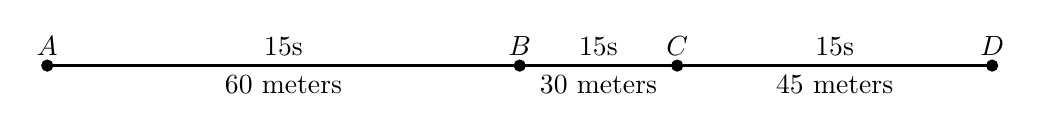
\begin{tikzpicture}
% Define the total length and segment lengths
\def\totalLength{12}
\def\segmentOne{6}   % 15s segment
\def\segmentTwo{2}   % 5s segment  
\def\segmentThree{4} % 10s segment

% Draw the main line
\draw[thick] (0,0) -- (\totalLength,0);

% Define the points
\coordinate (A) at (0,0);
\coordinate (B) at (\segmentOne,0);
\coordinate (C) at (\segmentOne+\segmentTwo,0);
\coordinate (D) at (\totalLength,0);

% Draw solid points at A, B, C, D
\foreach \point/\label in {A/A, B/B, C/C, D/D} {
    \filldraw[black] (\point) circle (2pt);
    \node[above] at (\point) {$\label$};
}

% Add time labels above the segments
\node[above] at ($(A)!0.5!(B)$) {15s};
\node[above] at ($(B)!0.5!(C)$) {15s};
\node[above] at ($(C)!0.5!(D)$) {15s};

% Optional: Add distance markers below the line
\node[below] at ($(A)!0.5!(B)$) {60 meters};
\node[below] at ($(B)!0.5!(C)$) {30 meters};
\node[below] at ($(C)!0.5!(D)$) {45 meters};


\end{tikzpicture}
  \end{center}
  \begin{enumerate}
    \item
	What is the formula of harmonic mean? \hfill 1
    \item
	When should we use the harmonic mean? \hfill 2
    \item  
	Find the average velocity of the vehicle. \hfill 3
    \item
	Compare the average speed estimated using the arithmetic and harmonic mean and \\ verify their suitability in the given situation. \hfill 4
  \end{enumerate}


 \item
	  \textbf{While driving from city A to city B, a car got 22 miles per gallon and
while returning on the same road, the car got 30 miles per gallon.} 
  \textcolor{red}{REVIEW THE QUESTION}
  \begin{enumerate}
    \item
	How many measures of centrtal tendencies are there? \hfill 1
    \item
	Which route takes more amount of fuel per mile? \hfill 2
    \item  
	If the total distance for the round trip was 300 miles, how many gallons of fuel were used for the entire journey? \footnote{$$\frac{150}{22} + \frac{150}{30} \text{ gallons} = \frac{130}{11} \text{ gallons} = 11.82 \text{ gallons}$$} \hfill 3
    \item
	Find the car’s average gas mileage for the entire trip, in miles per gallon. \hfill 4
  \end{enumerate}

     \item
	  \textbf{A shrimp producer wanted to get an insight into his shrimp production. To do so, he randomly collected weights of different shrimps in his farm.} 
	  

	  \begin{table}[h]
	  \centering
\begin{tabular}{c|c|c|c|c|c}
Weight of shrimp (gm) & 10-20 & 20-30 & 30-40 & 40-50 & 50-60 \\ \hline
Frequency & 5 & 8 & 10 & 9 & 4
\end{tabular}
\end{table}

  \begin{enumerate}
    \item
	What is the primary goal of central tendency?\hfill 1
    \item
	When is Median a better measure of central tendency than Arithmetic Mean and why? \hfill 2
    \item  
	From the stem, find 3rd quartile and explain. \hfill 3
    \item
	Find harmonic mean (HM) and compare with the arithmetic mean (AM) \hfill 4
  \end{enumerate}

 \item
	  \textbf{An arithmetic series is formed as follows:}
	  
	   \begin{center}
  \textbf{$a, a+c, a+2c, \cdots, a+2nc$}
  \end{center}
  
  \begin{enumerate}
    \item
	What is change of origin and scale? \hfill 1
    \item
	Convert the series into a set of natural numbers. \hfill 2
    \item  
	Find the arithmetic mean of the series with the use of change of origin and scale. \hfill 3
    \item
	Find the geometric mean of the series: $1, 2, 4, \cdots , 2^n$ . \hfill 4
  \end{enumerate}

 \item
	  \textbf{Scores by Travis Head in the last two matches of ICC Men's 
	  Cricekt World - 2023 are given. In Cricket, Strike Rate (SR) is computed by dividing Runs by Balls and then multiplying the quotient by 100.} 
	  
	  \begin{table}[h]
	  \centering
\begin{tabular}{c|c|c}
Match & Runs & Balls \\ \hline 
1 & 62 & 48 \\
2 & 137 & 120 \\ \hline 
\end{tabular}
\end{table}
  
  \begin{enumerate}
    \item
	How many averages do you know of? \hfill 1
    \item
	Give an example when arithmetic mean is appropriate instead of harmonic mean. \hfill 2
    \item  
	When is Weighted Harmonic mean is used. Show a numerical example. \hfill 3
    \item
	Determine the average Strike Rate of the batter \hfill 4
  \end{enumerate}
  
   \item
	  \textbf{Average height of the four tallest towers in Dhaka is 153.25 meters. The heights of first three towers is 171, 153 and 152 meters, respectively. A new tower has been built with height 150 meters.} 
  
  \begin{enumerate}
    \item
	Write two primary uses of central tendency. \hfill 1
    \item
	Prove mathematically: $\displaystyle \sum_{i=1}^n (x_i-\bar x) = 0$ \hfill 2
    \item  
	Compute the height of the forth tower. \hfill 3
    \item
	After the addition of the new tower, will the average increase or decrease? Explain logically and empirically (using data). \hfill 4
  \end{enumerate}

 \item
	  \textbf{For two non-zero positive numbers, $GM=4\sqrt3$ and $HM=6$, where the quantities bear usual notations} 
  
  \begin{enumerate}
    \item
	When is Harmonic mean suitable? \hfill 1
    \item
	For two numbers, what is the relationship between AM, GM, and HM? \hfill 2
    \item  
	What is the Arithmetic mean? \hfill 3
    \item
	Determine the numbers. \hfill 4
  \end{enumerate}
  
  \item
\textbf{For two positive non-zero numbers, if $GM = 5\sqrt{2}$ and $AM = 8$, where the symbols represent their usual meanings:}

\begin{enumerate}
    \item  
    Find the Harmonic mean (HM). \hfill 3
    \item
    Identify the two numbers. \hfill 4
\end{enumerate}

\item
\textbf{For two positive non-zero numbers, if $GM = 6\sqrt{3}$ and $AM = 10$, where the symbols represent their usual meanings:}

\begin{enumerate}
    \item  
    Determine the Harmonic Mean (HM) of the two numbers. \hfill 3
    \item
    Find the values of the two numbers. Comment on the obtained values. \hfill 4
\end{enumerate}

  
   \item
	  \textbf{12 is deducted from each value of a variable and then divided by 3. The new arithmetic mean (AM) is found to be 4.} 
  
  \begin{enumerate}
    \item
	What is change of origin? \hfill 1
    \item
	Does AM depend on origin? Prove with an example. \hfill 2
    \item  
	From the stem, find the original AM. \hfill 3
    \item
	Does the origin or the scale have greater impact on AM in this example? \hfill 4
  \end{enumerate}
  
   \item
	  \textbf{A statistics teacher gave a test to students worth 50 marks. After publishing the result, it was decided the marks would be converted to 100-marks scale. It was also noted that each student should get 2 marks more than the given marks.} 
  
  \begin{enumerate}
    \item
	In the stem, which concept is revealed? \hfill 1
    \item
	Does the arithmetic mean depend upon change of scale? \hfill 2
    \item  
	Demonstrate the effect of change of origin and scale on arithmetic mean, deriving the formula for conversion between them. \hfill 3
    \item 
    If the original arithmetic mean of the marks of the students is 44, what is the changed mean? Does the change of origin and scale always increase the value? Analyze.
	 \hfill 4
  \end{enumerate}

   \item
	  \textbf{The arithmetic and geometric means of ages two boys Abir and Abid are 10 and 8.} 
  
  \begin{enumerate}
    \item
	What is arithmetic mean? \hfill 1
    \item
	When can we not calculate arithmetic mean? \hfill 2
    \item  
	Determine the ages of Abir and Abid. \hfill 3
    \item
	Does the data comply with the theorem $\displaystyle AM \times  = GM^2$? \hfill 4
  \end{enumerate}
  
     \item
	  \textbf{Income of 100 individuals in the city of Rajshahi were analyzed and found to produce the the following distribution:} 
	  
	  \begin{table}[h]
	  	  \centering
\begin{tabular}{c|ccccc}
Income                                                           & 40-50 & 50-60 & 60-70 & 70-80 & 80-90 \\ \hline
\begin{tabular}[c]{@{}c@{}}Number of \\ Individuals\end{tabular} & 15    & 20    & 35    & 20    & 10   
\end{tabular}
\end{table}
  
  \begin{enumerate}
    \item
	What is Median? \hfill 1
    \item
	Does median necessarily lie in the dataset? \hfill 2
    \item  
	Estimate Median and explain the result. \hfill 3
    \item
	Find Arithmetic Mean and Mode. Which measure seems to be the best one? \hfill 4
  \end{enumerate}
  
   \item
	  \textbf{Amount of rainfall in some cities around the world for a month were obtained as follows:} 
	  
	      \begin{table}[h]
    \centering
\begin{tabular}{c|c}
\textbf{Rainfall (mm)} & \textbf{Frequency} \\ \hline
20-30                  & 5                  \\ \hline
30-40                  & 6                  \\ \hline
40-50                  & 4                  \\ \hline
50-60                  & 3                  \\
60-70                  & 5                 
\end{tabular}
\end{table}

    \begin{enumerate}
    \item
	When is Short-Cut method for Arithmetic Mean useful? \hfill 1
    \item
	Derive the formula of Short-cut Method \hfill 2
    \item  
	Compute the Arithmetic Mean using the Short-cut method. \hfill 3
    \item
	Compute the Arithmetic Mean with a different value of origin (a). Do both the methods give same result?\hfill 4
  \end{enumerate}
  
     \item
\textbf{The number of hours spent studying per week by students in a school were recorded as follows:}

\begin{table}[h]
\centering
\begin{tabular}{c|c}
\textbf{Hours Studied} & \textbf{Frequency} \\ \hline
0-5                   & 8                  \\ \hline
5-10                  & 12                 \\ \hline
10-15                 & 10                 \\ \hline
15-20                 & 6                  \\ \hline
20-25                 & 4                 
\end{tabular}
\end{table}

    \begin{enumerate}
    \item
	Relate short-cut method of arithmetic mean with change of origin and scale. \hfill 2
    \item  
	Compute the Arithmetic Mean of the given data using the short-cut method. \hfill 3
    \item
	Compute the Arithmetic Mean with a different value of origin (a). Do both the methods give same result? What is the best choice of a? \hfill 4
  \end{enumerate}
  
  \item
\textbf{Concentrations of a chemical solution (in mol/L) were recorded over 
several trials as follows:} 

\begin{table}[h]
\centering
\begin{tabular}{c|ccccc}
\textbf{Concentration (mol/L)} & 0.1-0.2 & 0.2-0.3 & 0.3-0.4 & 0.4-0.5 & 0.5-0.6 \\ \hline
\textbf{Frequency}             & 4       & 7       & 5       & 6       & 3       
\end{tabular}
\end{table}

\begin{enumerate}
    \item  
    Compute the Arithmetic Mean using the Short-cut method. \hfill 3
    \item
    Compute the Arithmetic Mean using a different assumed mean (A). \\
    Do both methods yield the same result? \hfill 4
\end{enumerate}

  
     \item
	  \textbf{A sports analyst collected ages of athelets having ages between 10 and 35. He then presented his findings as below:} 
	  
	  \begin{table}[h]
	    \centering
\begin{tabular}{c|c|c|c|c|c}
Age            & 10-15 & 15-20 & 20-25 & 25-30 & 30-35 \\ \hline
No. of Athlete & 2     & 8     & 10    & 5     & 3    
\end{tabular}
\end{table}
  
  \begin{enumerate}
    \item
	What is central tendency? \hfill 1
    \item
	When is geometric mean iappropriate to measure? \hfill 2
    \item  
	Compute median from the stem. \hfill 3
    \item
	Show that Arithmetic mean is greater than Harmonic mean. Which one of them is more suitable for this data? \hfill 4
  \end{enumerate}

   \item
	  \textbf{Mean monthly salaries of employees of two companies A \& B are tk. 
	  65,000 and tk. 75,000. The combined arithmetic mean (AM) is tk. 
	  71,000 and number of employees in the company A is 20.} 
	  
  \begin{enumerate}
    \item
	Write down the formula of combined AM for k groups. \hfill 1
    \item
	What is the combined AM of two data sets with AM 35 and 45 and number of values equal? \hfill 2
    \item  
	How many employees are there in the company B? \hfill 3
    \item
	Salary of an employee of company A was recorded as tk. 60,000 in place of
	65,000. What is the new AM of company A. Also find the corrected combined AM.\hfill 4
  \end{enumerate}
  
  \item
\textbf{Average marks of two sections A \& B in a statistics exam are 68 and 74 respectively. The overall average mark of both sections combined is 70. Section A has 25 students.}

\begin{enumerate}
    \item  
    How many students are there in section B? \hfill 3
    \item
    Later, it was found that a student in section B was wrongly marked 80 instead of 90. Find the corrected average of section B and the new combined average. \hfill 4
\end{enumerate}


     \item
	  \textbf{A departmental store records their sales. An analysis of products with prices less than tk. 30 generates the following table.} 
	  
\begin{table}[H]
\centering
\begin{tabular}{c|c|c|c|c|c|c}
Price     & 0-5 & 5-10 & 10-15 & 15-20 & 20-25 & 25-30 \\ \hline
Frequency & 1   & 0    & 2     & 3     & 8     & 12   
\end{tabular}
\end{table}
  
  \begin{enumerate}
    \item
	What is relative frequency? \hfill 1
    \item
	If $Y = a + bX$, $\bar Y = ?$ \hfill 2
    \item  
	Find 67th Percentile and 3rd Quartile and explain. \hfill 3
    \item
	Is AM or Median more suitable for this data? Elucidate. \hfill 4
  \end{enumerate}

   \item
	  \textbf{Arithmetic (AM) and Harmonic Mean (HM) of two numbers are 25 and 9, respectively.} 
    \begin{enumerate}
    \item
	When is HM useful? \hfill 1
    \item
	Derive HM formula using the concept of average velocity. \hfill 2
    \item  
	Find the two values from the stem. \hfill 3
    \item
	Show mathematically that $HM \le AM$ (for n=2) \hfill 4
  \end{enumerate}

   \item
  \textbf{Frequency distribution of marks in statistics of a college is given in the following table.}
 

\begin{table}[h]
\centering
\begin{tabular}{c|c|c}
\hline
Marks & \begin{tabular}[c]{@{}c@{}}Number of Students\\ Group - A\end{tabular} & \begin{tabular}[c]{@{}c@{}}Number of Students\\ Group - B\end{tabular} \\ \hline
25-30 & 11 & 10 \\ \hline
30-35 & 18 & 16 \\  \hline
35-40 & 21 & 22 \\ \hline
40-45 & 26 & 28 \\ \hline
45-50 & 14 & 9 \\ \hline
\end{tabular}
\end{table}

  \begin{enumerate}
    \item
	What is data? \hfill 1
    \item
	What are the disadvantages of secondary data? \hfill 2
    \item  
	Calculate the arithmetic mean of Group - A \hfill 3
    \item
	Compute the combined mean. Is it greather than the arithmetic mean of Group - B? Explain the possible reason(s). \hfill 4
\end{enumerate}

\item  
  \textbf{The following table presents the distribution of monthly salaries (in thousand BDT) of employees in two different departments of a company.}  

\begin{table}[h]
\centering
\begin{tabular}{ccc}
\hline
Salary Range (in 1000 BDT) & \begin{tabular}[c]{@{}c@{}}Number of Employees\\ Department - X\end{tabular} & \begin{tabular}[c]{@{}c@{}}Number of Employees\\ Department - Y\end{tabular} \\ \hline
20-25 & 8 & 6 \\ 
25-30 & 14 & 12 \\ 
30-35 & 19 & 21 \\ 
35-40 & 24 & 26 \\ 
40-45 & 15 & 10 \\ \hline
\end{tabular}
\end{table}

  \begin{enumerate}
    \item  
	Determine the arithmetic mean salary of employees in Department - X.  \hfill 3  
    \item  
	Compute the combined mean salary. Is it higher than the arithmetic mean of Department - Y? Justify your answer with a statistical explanation.  \hfill 4  
\end{enumerate}  



    \item
  \textbf{In the test examination, marks of 11 students in statistics are: 90, 92, 93, 49, 44, 88, 80, 58, 83, 71, 76.}
  \begin{enumerate}
    \item
	What is central tendency? \hfill 1
    \item
	When is median better than arithmetic mean? Explain with an example. \hfill 2
    \item  
	Find the 3rd the quartile and $61^{st}$ percentile from the data and explain.  \hfill 3
    \item
	Do quantiles depend on change of origin and scale. Prove using two examples.\hfill 4
\end{enumerate}

 \item
	  \textbf{HSC exam result of two colleges in a village are given below:} 
	  
	  \begin{table}[h]
	  \centering
\begin{tabular}{c|c|c}
College & Students & Passed \\ \hline
1 & 10 & 8 \\ \hline
2 & 20 & 5
\end{tabular}
\end{table}
  
  \begin{enumerate}
    \item
	How many measures of central tendency are there? \hfill 1
    \item
	Which measure of central tendency is perfect? \hfill 2
    \item  
	Find the pass rate of the colleges and, using them, of the village. \hfill 3
    \item
	Show an alternative method which gives the same result. \hfill 4
  \end{enumerate}

      \item
  \textbf{Scores of a batsman in the last 20 innings are} 
   \begin{center}
  	 28, 30, 16, 48, 50, 86, 105, 20, 10, 36, \\
  	 12, 25, 20, 35, 65, 12, 10, 76, 55, 32
  	 \end{center}
  \begin{enumerate}
    \item
	Write down the formula of weighted harmonic mean \hfill 1
    \item
	Can median be a better measure of central tendency than arithmetic mean for this data?  \hfill 2
    \item  
	Draw a stem and leaf plot from the data and explain.  \hfill 3
    \item
	Make a frequency distribution from the data and also find and interpret cumulative  \hfill 4 \\ frequencies and percentages.
\end{enumerate}

 \item
	  \textbf{In ODI cricket, two top batsmen are (as of 2nd Sept, 2022) Babar Azam and Rassie van der Dussen. Their average (arithmetic mean) scores are 59.79 and 69.32, appearing in 90 (including being not out in 12 occassions) and 33 (including being not out in 11 occassions) matches, respectively.} 
  
  \begin{enumerate}
    \item
	When is arithmetic mean inappropriate to use? \hfill 1
    \item
	Is arithmetic mean always suitable for comparison? \hfill 2
    \item  
	Find the combined arithmetic mean and explain. \hfill 3
    \item
	How to compare two sets of data having significantly distinct ranges? \hfill 4
  \end{enumerate}
  
   \item
	  \textbf{A fridge manufacturing company observe temperatures of newly developed 8 deep fridges. The observed temperatures (in degree celsius are:} 
	  
	    \begin{center}
-10, -8, -2, -4, -4, -1, -12, -3, -13
  \end{center}
  
  \begin{enumerate}
    \item
	What is a Decile? \hfill 1
    \item
	How many Deciles does a data set have? Why? \hfill 2
    \item  
	Compute the 8th Decile from the data and explain. \hfill 3
    \item
	Find and compare arithmetic and geometric mean from the data. \hfill 4
  \end{enumerate}
  
   \item
	  \textbf{Given below is a series of data.} 
	  
	  	    \begin{center}
	 $5, 7, 9, \cdots , 123$
	    \end{center}
  
  \begin{enumerate}
    \item
	What is the summation of natural numbers up to nth value? \hfill 1
    \item
	Find the arithmetic mean of natural numbers from 1 up to 20. \hfill 2
    \item  
	Find the arithmetic mean of the given series. \hfill 3
    \item
	Prove that arithmetic mean is greater than gemetric mean theoretically and empricially. \hfill 4
  \end{enumerate}
  
   \item
	  \textbf{Grades of a an undergraduate student with major in statistics are given below: } 
	  
	  [Credits serve as weights]

\begin{table}[h]
\centering
\begin{tabular}{c|c|c|c|c|c|c}
\hline
Course & Probability & Simulation & Calculus & Linear Algebra & Econometrics & Programming \\ \hline
Grade & 3.75 & 3.50 & 3.50 & 3.75 & 3.00 & 3.50 \\  \hline
Credit & 4 & 3 & 4 & 4 & 2 & 3 \\ \hline
\end{tabular}
\end{table}


  \begin{enumerate}
    \item
	Write down the formula of weighted mean. \hfill 1
    \item
	What is difference between weight and frequency? \hfill 2
    \item  
	Determine the GPA of the student. \hfill 3
    \item
	Determine the geometric mean for the data and evaluate \\ suitability. \hfill 4
  \end{enumerate}

 \item
	  \textbf{A student walks 3 hours at 5 km per hour (kph), 4 hours at 4 kph, and 2 hours at 3 kph.} 
  
  \begin{enumerate}
    \item
	When is harmonic mean suitable? \hfill 1
    \item
	Which mean could we use for the given data and why? \hfill 2
    \item  
	Find the average speed using weighted harmonic mean. \hfill 3
    \item
	Find the correct and suitable average speed using another method and mathematically show they are equivalent. \hfill 4
  \end{enumerate}
  
  \item
    \textbf{Scores of four athletes in different events at a track meet are recorded below:}

\begin{table}[h]
\centering
\begin{tabular}{c|c|c|c|c}
\hline
Event & High Jump & Long Jump & Shot Put & Javelin Throw \\ \hline
Score & 8.5 & 7.2 & 12.8 & 55.5 \\ \hline
Difficulty Factor & 2 & 3 & 2.5 & 1.5 \\ \hline
\end{tabular}
\end{table}

\textbf{A coach believes that events with higher difficulty factors should contribute more to the overall ranking and suggested a new weighting where the weight for each event is the square of its difficulty factor.}

  \begin{enumerate}
    \item
	Write down the formula of weighted mean. \hfill 1
    \item
	What is difference between weight and frequency? \hfill 2
	 \item Calculate the weighted average score of the athletes across all four events. \hfill 3
    \item If the coach's suggestion is implemented, would the mean be shifted upward or downward? Show mathematically and empricially. \hfill 4
  \end{enumerate}
  
  \item
\textbf{A biologist observes three different species of fish swimming at 
different speeds. The recorded swimming speeds are 2 m/s for 4 hours, 
3 m/s for 3 hours, and 5 m/s for 2 hours.}

\begin{enumerate}
    \item  
    Find the average swimming speed using the weighted harmonic mean. \hfill 3
    \item
    Confirm the average speed by applying another method and prove their 
    mathematical equivalence. \hfill 4
\end{enumerate}

\item
\textbf{A biologist records the lengths (in cm) of a certain species of 
fish found in different water bodies as shown below:}

\begin{table}[h]
\centering
\begin{tabular}{c|c|c|c|c|c}
\textbf{Category} & 5-10 & 10-15 & 15-20 & 20-25 & 25-30 \\ \hline
\textbf{Frequency} & 8    & 12    & 15    & 10    & 5     
\end{tabular}
\end{table}

\begin{enumerate}
    \item  
    Compute the Arithmetic Mean of the fish lengths. \hfill 3
    \item
    Suppose there is another set of data from a similar study with a mean of 17 cm and 20 observations. Find the combined mean of the two datasets and compare it with the mean found in (i). \hfill 4
\end{enumerate}

 \item
	  \textbf{A meteorologist records the monthly rainfall (in mm) in different regions over a year as shown below:}

\begin{table}[h]
\centering
\begin{tabular}{c|c|c|c|c|c}
\textbf{Rainfall (mm)} & 0-50 & 50-100 & 100-150 & 150-200 & 200-250 \\ \hline
\textbf{Frequency}     & 6    & 10     & 14      & 8       & 7       
\end{tabular}
\end{table}

  
  \begin{enumerate}
    \item
	Which class contains the Mode? \hfill 1
    \item
	Find $\Delta_1$ and $\Delta_2$, where the symbols represent their usual meanings \hfill 2
    \item  
	Find the Mode using the Direct formula. \hfill 3
    \item
	Find the Mode using histogram and compare with direct method. \\ Which one do you think is more accurate? \hfill 4
  \end{enumerate}
  
  
   \item
	  \item
\textbf{An ecologist records the number of trees in different forest plots based on their heights (in meters) over a survey period as shown below:}

\begin{table}[h]
\centering
\begin{tabular}{c|c|c|c|c|c}
\textbf{Tree Height (m)} & 0-5 & 5-10 & 10-15 & 15-20 & 20-25 \\ \hline
\textbf{Frequency}       & 5   & 12   & 18    & 9     & 6      
\end{tabular}
\end{table}

  
  \begin{enumerate}
    \item
	How much data lie below the Median point? \hfill 1
    \item
	What is the relationship between the median and the quartiles? \hfill 2
    \item  
	Find the median using the direct formula. \hfill 3
    \item
	Find the 1st and 3rd quartile from the table and interpret. \hfill 4
  \end{enumerate}
  
  \textcolor{red}{ADD QUESTIONS ASKING MODE AND MEDIAN AND OTHER QUARTILES FROM GRAPH}

\item
\textbf{A botanist measures the heights (in cm) of plants from a sample as shown below:}

\begin{table}[h]
\centering
\begin{tabular}{c|c|c|c|c|c}
\textbf{Height (cm)} & 20-30 & 30-40 & 40-50 & 50-60 & 60-70 \\ \hline
\textbf{Frequency} & 6 & 10 & 12 & 8 & 4
\end{tabular}
\end{table}

\begin{enumerate}
    \item  
    Find the median height of the plants and interpret. \hfill 3
    \item
    Determine the first (Q1) and third (Q3) quartiles of the plant heights. Explain the significance of these quartiles in understanding the data distribution. \hfill 4
\end{enumerate}

  
   \item
	  \textbf{A passer-by walks 3 hours at 5 km per hour (kph), another 3 hours 
	  at 4 kph, and another 3 hours at 3 kph.} 
  
  \begin{enumerate}
    \item
	When is harmonic mean suitable? \hfill 1
    \item
	Which mean could we use for the given data and why? \hfill 2
    \item  
	Find the average speed of the passer-by usingt he proper method. \hfill 3
    \item
	Find the correct and suitable average speed using another method and mathematically show they are equivalent. \hfill 4
  \end{enumerate}

 \item
	  \textbf{A cyclist moves around a square-shaped lake with the speeds 20, 25, 30, and 16 km per hour.} 
  
  \begin{enumerate}
    \item
	What is grouped data? \hfill 1
    \item
	Is arithmetic mean suitable for this data? \hfill 2
    \item  
	Find the average speed of the cyclist. \hfill 3
    \item
	Can we use some other formula for finding the same value of the average? Demonstrate. \hfill 4
  \end{enumerate}
  
     \item
	  \textbf{There are only two students in a class IX in a college. In half-yearly exam, the arithmetic and the geometric mean of the marks of those two studnets are 25 and 15, respectively.} 
  
  \begin{enumerate}
    \item
	Write down the formula of Geometric Mean for grouped data. \hfill 1
	\item Prove with an example: $\displaystyle \sum_{i=1}^n (x_i-\bar x) = 0$ \hfill 2
    \item  
	Determine the marks of the students. \hfill 3
    \item
	Is 20 a possible value of the harmonic mean of this data? Explain theoretically and empirically. \hfill 4
  \end{enumerate}

\begin{table}[h]
\centering
\begin{tabular}{c|c|c|c|c|c}
\textbf{Rainfall (mm)} & 20-30 & 30-40 & 40-50 & 50-60 & 60-70 \\ \hline
\textbf{Frequency} & 5 & 6 & 4 & 3 & 5
\end{tabular}
\end{table}
\end{enumerate}

\section{Short Questions}

\begin{enumerate}

\subsection{General Questions}

    \item What is the primary purpose of central tendency? \hfill 1
    \item When is WAM equal to WHM? Show mathematically. \hfill 2
    \item When is the equality true: $AM=GM=HM$? Prove mathematically and empirically.  \hfill 3
    \item When is Median a better measure of central tendency than Arithmetic Mean?  \hfill 1
    \item When is Harmonic Mean more suitable than Arithmetic Mean?  \hfill 1
    \item Write two primary uses of central tendency. \hfill 1
    \item For two distinct non-zero values, what is the relationship among AM, GM, and HM? \hfill 1
    \item what is the relationship among AM, GM, and HM? \hfill 1
    \item What are the criteria of a good measure of central tendency? \hfill 1
    \item For two non-zero positive numbers, prove $AM \ge GM \ge HM$ \hfill 3
    \item Find the AM, GM, and HM: $1,2,4,\cdots, 2^n$ \hfill 4
    \item A data set has the following values: 5, 10, 20, 30. Find AM, GM, HM, Median, and Mode and order the results in ascending order. \hfill 4

    
\subsection{Arithmetic Mean}

    \item Does Arithmetic Mean depend on change of origin and 
    scale? Prove mathematically and with an example. \hfill 3
    \item If $\bar{X} = 3 , \text{ and } n = 10$, what is $\sum X_i$? \hfill 2
    \item Derive the formula of combined mean using logic and an example. \hfill 2
    \item Prove with an example: $\displaystyle \sum_{i=1}^n (x_i-\bar x) = 0$ \hfill 2
    \item Prove mathematically: $\displaystyle \sum_{i=1}^n (x_i-\bar x) = 0$ \hfill 2
    \item Derive the formula of Arithmetic Mean for short-cut method. \hfill 2
    \item Derive the formula of combined Arithmetic Mean for $n$ nnumber of observations.
    \item Find Arithmetic Mean of first n natural numbers.
    \item If $u_i = x_i + y_i$, find $\bar x$ in terms of $u$. \hfill 1
    \item For two numbers, $AM=25$ and $GM=15$. $HM=?$ \hfill 1
    \item $\bar X = 25$ and $Y_i = 5X_i + 20$. $\bar Y = ?$
    \item Find Arithmetic Mean: $11,13,15, \cdots, 57$
    \item Find Arithmetic Mean: $115,120,125, \cdots, 225$
    \item Find Arithmetic Mean: $14,18,22, \cdots, 70$ \hfill 2
    \item Find Arithmetic Mean: $0, 5, 10, \cdots, 70$ \hfill 2
    \item Arithmetic Mean ($\bar X$) of five numbers is 40, and of three of them is 30. What is $\bar X$ of the rest two?
    \item AM of 200 values is found to be 50. Later it was seen two values were recorded as 92 and 8 in place of 192 and 88, respectively. What is the correct AM?
    \item AM of 8 values of 20. If the 9th value is 0, what is the new AM?
    \item AM of Income of City A is 1500 and of City B is 1200. If a person moves from city A to city B, can AM of both cities decrease?
    \item Calculate Arithmetic Mean:
    
    \begin{table}[h]
    \centering
\begin{tabular}{c|c}
\textbf{Renumeration (X)} & \textbf{No. of Employees (f)} \\ \hline
30               & 5                    \\ \hline
35               & 8                    \\ \hline
40               & 10                  
\end{tabular}
\end{table}
    
    \item Calculate Arithmetic Mean using short-cut method:
    
    \begin{table}[h]
    \centering
\begin{tabular}{c|c}
\textbf{Rainfall (mm)} & \textbf{Frequency} \\ \hline
20-30                  & 5                  \\ \hline
30-40                  & 6                  \\ \hline
40-50                  & 4                  \\ \hline
50-60                  & 3                  \\
60-70                  & 5                 
\end{tabular}
\end{table}

    \item What is the relationship between changing origin \& scale and short-cut method of Arithmetic Mean?

\subsection{Geometric Mean}    
    \item Write down the formula of Geometric Mean for grouped data.
    \item Find Geometric Mean for these values: $2, 4, 8$ \hfill 1
    \item Derive the formula of Geometric Mean using logarithm. \hfill 1
    \item When is Geometric Mean not calculable? \hfill 1
    \item When is Geometric Mean appropriate? \hfill 1
    \item Determine the formula of combined Geometric Mean when $n_1=n_2=n$ \hfill 1
    \item $Y_i = 3X_i$. If $G_y = 9, G_x=?$ [G stands for Geometric Mean] \hfill 2
    \item $n_1=15, G_1=75, n_2=10, \space and \space G_2=80$ Find combined GM.

\subsection{Harmonic Mean}

    \item Write down the formula of Weighted Harmonic Mean.\hfill 1
    \item When is Weighted Harmonic Mean used instead of Unweighted one? \hfill 1
    \item Calculate Harmonic Mean: $10,15,20$ \hfill 1
    \item Show mathematically that Harmonic Mean of velocity for a fixed distance is equal to average velocity.
    \item Find the average speed:
    
    \begin{table}[h]
    \centering
\begin{tabular}{c|c|c}
Path   & Distance (km) & Speed (km/h) \\ \hline
Path 1 & 3             & 8            \\ \hline 
Path 2 & 2             & 9            \\ \hline
Path 3 & 2             & 2           
\end{tabular}
\end{table}

\subsection{Median}

    \item Does Median depend on origin and scale? Prove with an example?
    \item How much data lie below the Median point? \hfill 1
    \item What is the relationship between the median and the quartiles? \hfill 2
    \item Median score of 50 students is 70. What does it mean? \hfill 1
    \item Write down the formula of Median for even number of observations.
    \item Write down the formula of Median for grouped data. 
    \item Find median: $5,10, 15, 20, 25, 30$
    \item Find median: $7,  2,  4,  5,  6, 10$ and explain the value \hfill 2
    \item Is Median affected by outliers?
    \item Does Median depend on origin and scale? Prove. \hfill 2
    \item What is the greatest disadvantage of Median?
    \item Does Median always lie in the data set from which it is calculated? \hfill 1
    
\subsection{Mode}

    \item What is the formula of Mode for grouped data?
    \item Find the mode: $2,2,3,3,4,4,2,2,7$
    \item What is an Unimodal dataset?

\subsection{Quadratic Mean}

    \item What is the formula of Quadratic Mean for grouped and ungrouped data?
    \item When is Quadratic Mean used?

\subsection{Partition Values}
    \item If a data is divided into four parts, how many partition values are created?
    \item Write down the formula of Median for even and odd number of observations.
    \item Derive the general formula of Quartiles using the concept of Median?
    \item Third Quartile of score of 50 students is 76. What does it mean?
    \item Which Quartile is equal to Median?
    \item Which Percentile is equal to 3rd Quartile?
    \item Find all the Quartiles and interpret: $2,1,0,5,-6,7,-4$ \hfill 3

    
\end{enumerate}

\chapter{Measures of Dispersion} 
\section{Creative Questions}

\begin{enumerate}
    \item
  \textbf{Temperatures of two cold regions for five days are as below:}

    \begin{center}

    City A: 2, 1, -1, 0, 3

    City B: 3, 0, -2, 2, 3
    
    \end{center}
  \begin{enumerate}
    \item
	What is standard deviation? \hfill 1
    \item
	Is standard deviation of a set of negative values negative? Justify mathematically. \hfill 2
    \item  
	Find Mean Deviation about mean of the values of city A.  \hfill 3
    \item
	Which city has more consistent weather? Verify statistically. \hfill 4
\end{enumerate}

\item  
  \textbf{Rainfall (in mm) recorded in two towns over five days is as follows:}

\begin{table}[h]
\centering
\begin{tabular}{c|ccccc}
Day     & 1  & 2  & 3  & 4  & 5  \\ \hline
Town X  & 12 & 15 & 10 & 18 & 14 \\
Town Y  & 20 & 22 & 18 & 25 & 21
\end{tabular}
\end{table}


  \begin{enumerate}
    \item  
	Find the Mean Deviation about the median for the rainfall data of Town X.  \hfill 3  
    \item  
	Which town shows greater variability in rainfall? Support your answer with statistical measures.  \hfill 4  
\end{enumerate}

\item  
  \textbf{Scores of two students in five tests are as follows:}

\begin{table}[h]
\centering
\begin{tabular}{c|ccccc}
Test     & 1  & 2  & 3  & 4  & 5  \\ \hline
Student A  & 78 & 85 & 90 & 88 & 76 \\ 
Student B  & 80 & 82 & 78 & 86 & 84
\end{tabular}
\end{table}

  \begin{enumerate}
    \item  
	Find the Mean Deviation about the mean for the scores of Student A.  \hfill 3  
    \item  
	Which student has more consistent performance? Justify using statistical measures.  \hfill 4  
\end{enumerate}  

\item  
  \textbf{Monthly sales (in thousand dollars) of two stores over five months are given below:}

\begin{table}[h]
\centering
\begin{tabular}{c|ccccc}
Month     & 1  & 2  & 3  & 4  & 5  \\ \hline
Store P  & 50 & 55 & 48 & 52 & 49 \\
Store Q  & 60 & 58 & 65 & 63 & 61
\end{tabular}
\end{table}

  \begin{enumerate}
    \item  
	Calculate the variance of Store P’s sales data.  \hfill 3  
    \item  
	Compare the sales stability of both stores using an appropriate statistical measure.  \hfill 4  
\end{enumerate}  


 \item
	  \textbf{Two companies A and B pay their workers on a weekly basis. The summary of wages paid by them is shown below:} 
	  
	  \begin{table}[h]
	  \centering
\begin{tabular}{c|ccc}
Factory & Wage (BDT) & Standard Deviation & Number of workers \\ \hline
A       & 1560       & 90                 & 200               \\ 
B       & 1580       & 70                 & 160              
\end{tabular}
\end{table}
  
  \begin{enumerate}
    \item
	What is dispersion? \hfill 1
    \item
	Is variance always greater than stanard deviation? Justify. \hfill 2
    \item  
	Which company is more consistent with their wages? \hfill 3
    \item
	Find the combined Coefficient of Variance (CV) and compare with individual companies. \hfill 4
  \end{enumerate}
  

 \item
	  \textbf{Mean and Standard Deviation of 200 items are found to be 60 and 20. Later it was found that two items were recorded as 3 and 67 in place of 13 and 17.} 
  
  \begin{enumerate}
    \item
	Does standard deviation depend on change of origin? \hfill 1
    \item
	Prove $\displaystyle \sigma^2 = \frac{\sum x^2}n -(\frac{\sum x}{n})^2$ from original formula. \hfill 2
    \item  
	Should the correct mean be smaller or greater? Also find it and compare.  \hfill 3
    \item
	Find the correct standard deviation. \hfill 4
  \end{enumerate}
      \item
  \textbf{The table below presents the number of goals scored by two footballers, A and B, over five consecutive seasons}

 \begin{table}[h]
\centering
\begin{tabular}{c|c|c|c|c|c}
Season      & 1  & 2  & 3  & 4  & 5  \\ \hline
Footballer A & 10 & 15 & 12 & 9  & 20 \\ \hline
Footballer B & 25 & 5  & 10 & 15 & 6  
\end{tabular}
\end{table}

  \begin{enumerate}
    \item  
	Find Mean Deviation about mean and median of the footballer A.  \hfill 3
    \item
	Which footballer should be hired a club? Determine with the help of a suitable relative measure of dispersion. \hfill 4
\end{enumerate}

\end{enumerate}

\section{Short Questions}

 \begin{enumerate}
 
 \item Which measure of dispersion is suitable for an open-ended distribution?  \hfill 1
 \item What does dispersion measure?  \hfill 1
 \item What are the absolute measures of dispersion?
 \item What are the relative measures of dispersion?
 \item What is the formula of Range? \hfill 1
 \item Does Range consider all values?
 \item Is Range influenced by extreme values or outliers? \hfill 1
 \item Write down the formula of Mean Deviation ($MD(\bar x)$.
 \item Write down the formula of Mean Deviation around median ($MD(Me)$.
 \item Write down the formula of Mean Deviation for grouped data ($MD(\bar X)$.
 \item Does mean deviation depend on all values of a dataset? \hfill 1
 \item Does Mean Deviation depend on change of origin and scale? Verify. \hfill 2
  \item When is variance less than standard deviation? \hfill 1
  \item Write down the formula of Quartile Deviation. \hfill 1
 \item Which is the most important measure of dispersion?
   \item Is $\sum |x_i-\bar x|$ always greater than $\sum (x_i-\bar x)$? Prove mathematically. \hfill 2
   \item If $\bar X = 25, CV = 50\%, \sigma^2=?$ \hfill 1
   \item Arithmetic mean of a variable is 16 and variance is 9. What is the value of CV? \hfill 1 
   \item What is the variance of first 5 natural numbers?
 
 \item Find the sum of squares: 12, 10, 11, 15, 20 \hfill 1
 \item Find the square of summation: 2, 5, 7, 8, 4 \hfill 1
 \item Find the sum of squared deviation from the mean of these values: 2, 5, 6, 7, 3 \hfill 1
 \item Find the sum of squares: 8, 6, 9, 12, 14 \hfill 1  

\item Find the square of summation: 3, 7, 5, 9, 6 \hfill 1  

\item Find the sum of squared deviation from the mean of these values: 4, 8, 6, 10, 7 \hfill 1  

\item Compute the sum of squares for the following values: 5, 9, 12, 14, 11 \hfill 1  

\item Compute the square of summation for: 1, 4, 6, 7, 2 \hfill 1  

\item Find the sum of squared deviations from the mean: 3, 6, 8, 10, 5 \hfill 1  

\item Find the sum of squares of differences from 10: 6, 8, 10, 12, 14 \hfill 1  



\subsection{Variance}
\item If $n=10, \sum x_i = 120, \sum x_i^2=2000, CV=?$
\item Is coefficient of variation a pure number? \hfill 1

\end{enumerate}


\chapter{Moments, SKewness, and Kurtosis} 
\section{Creative Questions}

  \begin{enumerate}
  
   \item
	  \textbf{The first four moments around 4 of productions of a company over four years are -1.5, 17, -30, and 108.} 
  
  \begin{enumerate}
    \item
	Can the second central moment be negative? \hfill 2
    \item  
	Determine the second and third central moments. \hfill 3
    \item
	What kind of kurtosis do the data have? \hfill 4
  \end{enumerate}

   \item
	  \textbf{Duration of stays of a spy in foreign countries are obtained by a researcher. As part of an analysis, s/he starts with the following summary.} 
	  
	  \begin{table}[h]
	  \centering
\begin{tabular}{c|cccccc}
Duration & 1-10 & 11-20 & 21-30 & 31-40 & 41-50 & 51-60 \\ \hline
Frequency & 4 & 3 & 3 & 2 & 5 & 2
\end{tabular}
\end{table}
  
  \begin{enumerate}
    \item
	What is symmetry? \hfill 1
    \item
	What is implied by the value of coefficient of skewness 0.8 \hfill 2
    \item  
	Estimate the median of the data and interpret. \hfill 3
    \item
	Obtain coefficient of skewness from data and comment on the life of the spy based on it. \hfill 4
  \end{enumerate}
  
   \item
	  \textbf{The kurtosis and the variance of a symmetrical distribution are $\gamma_2 = -2.3672$ and $\sigma^2 = 4096$, respectively.} 
  
  \begin{enumerate}
    \item  
	Find the fourth central moment. \hfill 3
    \item
	Determine the value of the first and the third raw moments around 5. \hfill 4
  \end{enumerate}
  
  \item  
\textbf{A human resources department recorded the number of years employees have been with the company. The grouped frequency distribution below summarizes the data for a department.}  

\begin{table}[h]
\centering
\begin{tabular}{c|c|c|c|c|c|c}
Years of Service & 0–2 & 3–5 & 6–8 & 9–11 & 12–14 & 15–17 \\ \hline
Frequency & 4 & 6 & 10 & 5 & 3 & 2
\end{tabular}
\end{table}

\begin{enumerate}
  \item  
  Calculate the coefficient of skewness using the grouped data. What does the result indicate about employee tenure? \hfill 3

  \item  
  Compute the coefficient of kurtosis. What does it reveal about the distribution of tenure lengths? \hfill 4
\end{enumerate}

  
  \item  
  \textbf{A financial analyst is studying the annual returns (in percentage) of a set of investment portfolios. The following table summarizes the data.}  

\begin{table}[h]
\centering
\begin{tabular}{c|cccccc}
Annual Return (\%) & -5 to 0 & 1-5 & 6-10 & 11-15 & 16-20 & 21-25 \\ \hline
Frequency & 3 & 5 & 7 & 6 & 4 & 3
\end{tabular}
\end{table}

  \begin{enumerate}
    \item  
	Compute the skewness of the data and interpret the nature of the investment returns.  \hfill 3  
    \item  
	Determine the kurtosis and explain.  \hfill 4  
  \end{enumerate}  



   \item
	  \textbf{There has been an increase in average lifetime of people of Bangladesh. To get more insight on this, a research was conducted, in which ages of retired government employees were recorded. A sample of 10 people is given below:}
	  
	  \begin{center}
	  75, 62, 63, 72, 66, 76, 59, 77, 70, 79
	  \end{center}
    \begin{enumerate}
    \item
	What is the 2nd central moment equal to? \hfill 1
    \item
	Show that the first central moment is zero. \hfill 2
    \item  
	Find the variance of the data. \hfill 3
    \item
	Are the data symmetric? Justify. \hfill 4
  \end{enumerate}
  
  \item
\textbf{A study was conducted to track the daily water consumption (in liters) 
of 10 individuals over a week. The recorded values are as follows:}

\begin{center}
2.5, 3.1, 2.8, 3.5, 2.7, 3.3, 2.6, 3.0, 2.9, 3.4
\end{center}

\begin{enumerate}
\item
Determine the variance of the data set. \hfill 3
\item
Assess whether the data distribution appears to be symmetric with the help
two different methods. \hfill 4
\end{enumerate}

\item  
\textbf{A researcher analyzed the daily screen time (in hours) of 12 students over a month. The recorded values are as follows:}  

\begin{center}  
4.2, 5.1, 3.8, 6.5, 4.7, 5.3, 4.6  
\end{center}  

\begin{enumerate}  
\item  
Compute the five-number summary of the data. \hfill 3  
\item  
Analyze the skewness of the dataset using both graphical and numerical approaches. \hfill 4  
\end{enumerate}  

  
   \item
	  \textbf{The arithmetic and geometric means of the first and third 
	  quartiles of a distribution are 10 and 8, respectively. The 
	  second quartile is 10.} 
  
  \begin{enumerate}
    \item
	What is the formula suggested by Pearson to find skewness? \hfill 1
    \item
	Which moments are useful in measuring central tendency and dispersion?  \hfill 2
    \item  
	Find skewness from the stem using a suitable formula. \hfill 3
    \item
	Which method of finding skewness od you think is the best and why? \hfill 4
\end{enumerate}

 \item
	  \textbf{For a particular data set, Median = 120, Mode = 110, Standard Deviation = 4, and Coefficient of Variation (CV)  = 3.2} 
  
  \begin{enumerate}
    \item
	Why is  CV used?  \hfill 1
    \item
	Find arithmetic mean.. \hfill 2
    \item  
	Find skewness according to Pearson's method ($SK_P$) \hfill 3
    \item
	Does ($SK_P$) convey the proper idea about the data as to the given information? Justify. \hfill 4
  \end{enumerate}
  
  \item
\textbf{For a given data set representing the monthly salaries (in thousands) of employees in a company, the following statistics are provided: Median = 60, Mode = 55, Standard Deviation = 5, and Coefficient of Variation (CV) = 8.3.}

\begin{enumerate}
    \item  
    Calculate the skewness using Pearson's method ($SK_P$). \hfill 3
    \item
    Does the value of ($SK_P$) accurately reflect the nature of the data based on the given statistics? Justify your answer. \hfill 4
\end{enumerate}


 \item
	  \textbf{US Dollar exchange (to taka) in Bangladesh since 1980 to 2005 (after each 5 years) were: \\ 16, 31, 36, 40, 52, 64} 
  
  \begin{enumerate}
    \item
	What are moments? \hfill 1
    \item
	Which moment is equal to the variance? Show mathematically. \hfill 2
    \item  
	Find, from the stem, the first and second raw moments about 1. \hfill 3
    \item
	Find skewness and kurtosis of and explain. \hfill 4
\end{enumerate}

 \item
	  \textbf{A farmer in Dinajpur district produces seasonal crops. First four moments around 9 of his daily earnings are computed as -1, 8, -16, and 25.}
  
  \begin{enumerate}
    \item
	What is the Box and Whisker plot? \hfill 1
    \item
	Can Box and Whisker plot suggest symmetry? \hfill 2
    \item  
	 Find the arithmetic mean and variance of the farmer's earnings.\hfill 3
    \item
	Do the earnings produce a symmetric data? Analyze. \hfill 4
  \end{enumerate}

 \item
	  \textbf{The first four moments about 3 of a distribution are -1, 5, -10, and 120.} 
  
  \begin{enumerate}
    \item
	What are moments used for? \hfill 1
    \item
	Can the second central moment be greater than the third central moment? \hfill 2
    \item  
	Find the second and third moments about arithmetic mean of the distribution. \hfill 3
    \item
	Find skewness and kurtosis and comment on the values.  \hfill 4
\end{enumerate}

  \item
	  \textbf{The first four moments of a distribution around 5 are 2, 20, 40, and 50, respectively.} 
  
  \begin{enumerate}
	\item 
	Draw the shape of a left-skewed distribution. \hfill 1
	\item 
	Derive the value of thew first central moment. \footnote{$\frac{\sum(x_i-\bar x}{n} = \bar x - \bar x) = 0$} \hfill 2
    \item
    Obtain the first four central moments. \hfill 3
    \item
	Estimate and comment on the skewness and kurtosis. \hfill 4
  \end{enumerate}
  
  \item
\textbf{A data set represents the test scores of 10 students in a recent exam, recorded as follows:}

\begin{center}
56, 62, 68, 71, 65, 59, 74, 67, 70, 63
\end{center}

\begin{enumerate}
\item
Calculate the first four moments \footnote{62.5, 3934.5, 249407.5, 15915069} about 3. \hfill 3
\item
Compute the variance and kurtosis of the data using converted central moments. 
Explain what the kurtosis indicates about the distribution. \hfill 4
\end{enumerate}


 \item
	  \textbf{Marks obtained by a student in 7 subjects are} 
	  \begin{center}
	  70, 66, 55, 45, 80, 30, 82
	\end{center}
  
  \begin{enumerate}
    \item
	What is negative skewness? \hfill 1
    \item
	Draw graphs of positive and negative skewness showing the locations of mean and median. \hfill 2
    \item  
	Determine the five number summary from the stem and explain. \hfill 3
    \item
	Are the data symmetric? If not, comment on the pattern of data. \hfill 4
\end{enumerate}

 \item
	  \textbf{United Nations Children's Fund (UNICEF) is an agency of the United Nations responsible for providing humanitarian and developmental aid to children worldwide. A  UNICEF researcher collected heights (in feet) of 7 children for a project, and the heights are} 

	\begin{center}
	  2.2, 2.15, 1.9, 3.1, 2.7, 3.0, 3.5
	  	\end{center}
  
  \begin{enumerate}
    \item
	Which value are central moments estimated around? \hfill 1
    \item
	Moments around origin (0) are central moments - Comment. \hfill 2
    \item  
	Find the first three central moments. \hfill 3
    \item
	Find the skewness of the data and interpret.  \hfill 4
  \end{enumerate}
  

  
   \item
	  \textbf{A researcher wants to compare average life time of people in Bangladesh and other countries. He collected life time of 10 people in Bangladesh.} 
	  
	  	\begin{center}
	  75, 62, 63, 72, 66, 76, 59, 77, 70, 79
	  	\end{center}
  
  \begin{enumerate}
    \item
	What is symmetry? \hfill 1
    \item
	Mathematically show the theoretical value of the first central moment. \hfill 2
    \item  
	Compute the 2nd, 3rd, and 4th central moments of the data. \hfill 3
    \item
	Estimate skewness and kurtosis and explain. \hfill 4
  \end{enumerate}
  
   \item
	  \textbf{Exam marks of two students were summarized for the purpose of comnparison. The summary is given below:} 
	  
	  \begin{table}[h]
	  \centering
\begin{tabular}{c|c|c}
Measure         & Student X & Student Y \\ \hline
First Quartile  & 28        & 27        \\
Second Quartile & 60        & 60        \\
Third Quartile  & 75        & 73        \\
Minimum         & 16        & 14        \\ 
Maximum         & 89        & 86        \\  \hline
\end{tabular}
\end{table}
  
  \begin{enumerate}
    \item
	What is kurtosis? \hfill 1
    \item
	How much data are contained within Interquartile range? \hfill 2
    \item  
	For student A, estimate the Bowley's Coefficient of skewness and explain. \hfill 3
    \item
	On the basis of skewness (and hence shape of the data), compare the students. \hfill 4
  \end{enumerate}
  
   \item
	  \textbf{The first four moments around 2 of a dataset were the following:}
	  
	  \begin{center}
	  \textbf{-1, 5, 20, 90}
	  \end{center}
  
  \begin{enumerate}
    \item
	What is raw moment? \hfill 1
    \item
	What is the standard deviation of the data in the stem? \hfill 2
    \item  
	Determine the third central moment. \hfill 3
    \item
	Comment on the kurtosis of the given data. \hfill 4
  \end{enumerate}
  
     \item
	  \textbf{The heights of the trees of a certain species that were planted at around the same time in a park were examined by an analyst, hired by the park authority to check for any abnormality. He randomly observed 10 trees; the values (in cm) obtained are given below:} 
	  
	  	  \begin{center}
	  \textbf{200, 190, 185, 210, 220, 200, 205, 207, 230, 195}
	  \end{center}
  
  \begin{enumerate}
    \item
	What is five number summary? \hfill 1
    \item
	Which measures are shown on a Box \& Whisker plot? \hfill 2
    \item  
	Display the data on a box plot. \hfill 3
    \item
	Taking a look at the drawn box plot, comment on the symmetry of the data. \hfill 4
  \end{enumerate}
  
  \item
\textbf{The weights of newborn babies (in kilograms) in a hospital over a week were recorded by a pediatrician to monitor their health. The weights of 10 randomly selected babies are given below:}

\begin{center}
\textbf{3.2, 2.9, 3.5, 3.1, 3.4, 3.0, 3.3, 3.6, 2.8, 3.7}
\end{center}

\begin{enumerate}
    \item  
    Represent the data using a Box \& Whisker plot. \hfill 3
    \item
    Compare the plot with the five-number summary and comment on the distribution of the data. \hfill 4
\end{enumerate}


\end{enumerate}

\section{Short Questions}
\begin{enumerate}
    \item What are moments? \hfill 1
    \item How many types of moments are there?  \hfill 1
    \item What is central moment? \hfill 1
    \item  What is raw moment? \hfill 1
    \item  What is the formula of raw moment for grouped data? \hfill 1
    \item Derive the value of the first central moment. \hfill 2
    \item  Derive the relationship between the first central moment and the origin.\hfill 2
    \item What is the second central moment equal to?\hfill 1
    \item Write 3 uses of moments.\hfill 2
    \item Can moments be negative? Analyze. \hfill 2
    \item What is skewness? \hfill 1
    \item What is a symmetric distribution? \hfill 1
    \item In a symmetric distribution, what is the relationship between Mean, Median, and Mode? \hfill 1
    \item What is negative skewness?\hfill 1
    \item What is positive skewness?\hfill 1
    \item What is the pattern of in a left-skewed didstribution?\hfill 2
    \item What is the pattern of in a right-skewed didstribution?\hfill 2
    \item In a left-skewed distribution, what is the relationship between Mean, Median, and Mode? \hfill 2
    \item In a right-skewed distribution, how \footnote{$Mo < Me < \bar X$} are Mean, Median, and Mode related?  \hfill 2
    \item Draw the shape of a left-skewed distribution and show locations of mean, median, and mode.  \hfill 2
    \item Draw the shape of a right-skewed distribution and show locations of mean, median, and mode.  \hfill 2
    \item Draw a symmetrical distribution.   \hfill 1
    \item Draw the shape of a right-skewed distribution.  \hfill 1
    \item What is Pearson's measure of skewness? \hfill 1
    \item How did Bowley measure skewness? \hfill 1
    \item What is Kelly's method of coefficient of skewness? \hfill 1
    \item How are moments used to mesure skewness?
    \item What is the relationship between $\beta_1$ and $\gamma_1$ \hfill 1
    \item What does $\gamma_1>0$ imply \hfill 1
    \item What is kurtosis? \hfill 1
    \item How many types of kurtosis are there? \hfill 1
    \item Draw the curve of a Mesokurtic distribution \hfill 1
    \item Draw the curve of a Platykurtic distribution \hfill 1
    \item Draw the curve of a Leptokurtic distribution \hfill 1
    \item Explain the Platykurtic distribution. \hfill 2
    \item How can you use moments to estimate kurtosis?
    \item What is the relationship between $\beta_2$ and $\gamma_2$
    \item What does $\gamma_2>0$ imply? \hfill 1
    \item What is five number summary?
    \item Find five number summary: 2, 1, 0, 5, -6, 7, -4 \hfill 3
    \item Write three uses of five number summary \hfill 2
    \item Which measures are shown on a Box \& Whisker plot?
    \item How is inner fence found for a Box \& Whisker plot
    \item How is outer fence found for a Box \& Whisker plot
    \item What is IQR and how is it calculated? \hfill 2
    \item Write four uses of the box plot. \hfill 2
    \end{enumerate}

\section{Broad Questions}
    \begin{enumerate}
    \item Analyze the effect of shift of origin \& scale on central moments. \hfill 3
    \item Prove that $\beta_1$ and $\beta_2$ do not depend on shift of origin and scale. \hfill 4
    \item Express the 3rd central moment in terms of raw moments. 
    \item The first four moments of a distribution around 5 are 2, 20, 40, and 50, respectively. Obtain the first four central moments. Estimate and comment on the skewness and kurtosis. 
    \end{enumerate}

\chapter{Correlation and Regression} 
\section{Creative Questions}

 \begin{enumerate}
 
  \item
	  \textbf{The temperature (in $^o$ Celsius) and rainfall (mm) in the city of Mymensingh on the last 6 rainingd days are summarized as below (temperature is denoted by $X$ and rainfall by $Y$: } 
	  
	  \begin{center}
	  $\sum x = 29, \sum y = 38, \sum xy = 205, \sum x^2 = 167, \sum y^2 = 282$
  \end{center}
  \begin{enumerate}
    \item
	What is covariance? \hfill 1
    \item
	Differentiate between cvariance and correlation. \hfill 2
    \item  
	Analyze the linear association between temperature and rainfall. \hfill 3
    \item
	Find the degree of impact of temperature on rainfall. \hfill 4
  \end{enumerate}
 
  \item
	  \textbf{The following table shows the exam scores of 10 students and the number of hours they studied for the exam. It is hypothesized that the exam score depends on the number of hours studied.} 
	  
\begin{table}[h!]
\centering
\begin{tabular}{c|c|c|c|c|c|c|c|c|c|c}
Hours Studied (X) & 2 & 3 & 4 & 5 & 6 & 7 & 8 & 9 & 10 & 11 \\ \hline
Exam Score (Y) & 65 & 70 & 72 & 78 & 80 & 85 & 88 & 92 & 95 & 98 \\
\end{tabular}
\end{table}
  
  \begin{enumerate}
    \item  
	Estimate and interpret the regression coefficient of y on x. \hfill 3
    \item
	Using data, show $r = \sqrt{b_{yx} \times b_{xy}}$; How much variation is explained by the obtained model? \hfill 4
  \end{enumerate}
\end{enumerate}

\section{Short Questions}

  \begin{enumerate}
  \item What does $r=-1$ imply? \hfill 1
  \item Does the regression coefficient depend on scale? Verify mathematically. \hfill 2
  \item What is the range of the correlation coefficient?  \hfill 1
  \item What is the range of the regression coefficient? \hfill 1
  \item What is the relationship between the regression coefficient and the correlation coefficient? \hfill 1
  \item What does $b_{yx} = 0.85$ imply? \hfill 1
  \item Two sets of variables have correlation $r_1 = 0.75$ and $r_2 = -0.82$. Which set has stonger linear association? \hfill 1
  \item How are correlation and regression different? \hfill 2
  \end{enumerate}

\chapter{Time Series} 
\section{Creative Questions}
  \begin{enumerate}
  
  \item
\textbf{The monthly sales (in units) of laptops at a major electronics store are recorded below:} 

\begin{table}[h]
\centering
\begin{tabular}{c|cccccccc}
\textbf{Month} & Jan & Feb & Mar & Apr & May & Jun & Jul & Aug \\ \hline
\textbf{Sales} & 120 & 150 & 130 & 170 & 160 & 180 & 200 & 210
\end{tabular}
\end{table}

\begin{enumerate}
  \item  
  Compute the trend using a three-monthly moving average method. \hfill 3
  \item
  Illustrate the trend graphically and estimate the expected laptop sales for September. \hfill 4
\end{enumerate}


   \item
	  \textbf{The yearly revenue (in hundred thousand) of shoe manufacturer company is given below} 
  \begin{table}[h]
\centering
\begin{tabular}{cccccccc}
Year     & 2005 & 2006 & 2007 & 2008 & 2009 & 2010 & 2011 \\ \hline
Revenue & 35   & 22    & 40     & 35     & 50     & 42 & 60   
\end{tabular}
\end{table}
  
  \begin{enumerate}
    \item
	What is general trend? \hfill 1
    \item
	Which method of determining trend gives only two values? \hfill 2
    \item  
	Determine the trend using three-yearly moving average method. \hfill 3
    \item
	Find the trend using graphical method and extrapolate the approximate revenue earned in 2012. \hfill 4
  \end{enumerate}
  
  \item
\textbf{The annual production (in thousand tons) of a steel manufacturing plant over seven years is given below:}

\begin{table}[h]
\centering
\begin{tabular}{cccccccc}
Year     & 2015 & 2016 & 2017 & 2018 & 2019 & 2020 & 2021 \\ \hline
Production & 50   & 55   & 60   & 65   & 70   & 75   & 80   
\end{tabular}
\end{table}

\begin{enumerate}
    \item  
    Compute the trend using the three-yearly moving average method. \hfill 3
    \item
    Estimate the approximate production for the year 2022 using both graphical and moving average methods. \hfill 4
\end{enumerate}

\item
\textbf{The average monthly temperature (in degrees Celsius) recorded at a weather station over seven months is given below:}

\begin{table}[H]
\centering
\begin{tabular}{c|c|c|c|c|c|c|c}
Month & September & October & November & December & January & February & March \\ \hline
Temperature & 22 & 20 & 18 & 15 & 12 & 16 & 20
\end{tabular}
\end{table}

\begin{enumerate}
\item
Compute the trend using the three-monthly moving average method. \hfill 3
\item
Estimate the approximate average temperature for the month of April using both graphical and moving average methods, and compare the projections. \hfill 4
\end{enumerate}

\item  
\textbf{The monthly rainfall (in mm) recorded in a city over seven consecutive months is given below:}  

\begin{table}[h]  
\centering  
\begin{tabular}{cccccccc}  
Month     & Jan  & Feb  & Mar  & Apr  & May  & Jun  & Jul  \\ \hline  
Rainfall (mm) & 85   & 42   & 78   & 150  & 210  & 95   & 180    
\end{tabular}  
\end{table}  

\begin{enumerate}  
    \item  
    Determine the trend using the three-month moving average method. \hfill 3  
    \item  
    Predict the expected rainfall for August using both graphical and moving average techniques. \hfill 4  
\end{enumerate}  


\item
\textbf{The annual sales (in million dollars) of a tech company over eight years are provided below:}

\begin{table}[h]
\centering
\begin{tabular}{ccccccccc}
Year     & 2014 & 2015 & 2016 & 2017 & 2018 & 2019 & 2020 & 2021 \\ \hline
Sales    & 120  & 150  & 140  & 160  & 180  & 200  & 220  & 240   
\end{tabular}
\end{table}

\begin{enumerate}
    \item  
    Calculate the trend using the three-yearly moving average method. \hfill 3
    \item
    Predict the approximate sales for the year 2022 using both graphical and moving average methods. \hfill 4
\end{enumerate}
  
  \item
\textbf{The monthly sales (in thousands of units) of a product for the last 6 months are given below:}

\begin{table}[h]
\centering
\begin{tabular}{ccccccc}
Month     & January & February & March & April & May & June \\ \hline
Sales     & 80      & 95       & 110   & 105   & 120  & 115  \\
\end{tabular}
\end{table}

\begin{enumerate}
\item
Determine the trend using the three-month moving average method. \hfill 3
\item
Plot the trend and forecast the sales for July using two methods 
and compare. \hfill 4
\end{enumerate}

\item
\textbf{The quarterly production data (in tons) for a factory is given below:}

\begin{table}[h]
\centering
\begin{tabular}{cccccccc}
Quarter    & Q1     & Q2     & Q3     & Q4     & Q5     & Q6     & Q7     \\ \hline
Production & 150    & 160    & 155    & 145    & 170    & 165    & 180    \\
\end{tabular}
\end{table}

\begin{enumerate}
\item
Calculate the trend using the moving average method for a 3-quarter period. \hfill 3
\item
Plot the trend line and predict the production for Q8 using two methods 
and compare. \hfill 4
\end{enumerate}


  
     \item
	  \textbf{Bangladesh foreign debt has been increasing rapidly in recent years. The Bangladesh bank provides the follwoing data.}
	  
	  \begin{table}[h]
	  \centering
\begin{tabular}{c|c|c|c|c|c|c|c|c|c}
Fiscal Year & 2015-16 & 2016-17 & 2017-18 & 2018-19 & 2019-20 & 2020-21 & 2021-22 & 2022-23 & 2023-24 \\ \hline
Debt & 41.17 & 45.81 & 56.01 & 62.63 & 68.55 & 81.62 & 95.45 & 98.94 & $\sim$130.00
\end{tabular}
\end{table}
  
  \begin{enumerate}
    \item
	Name the components of time series. \hfill 1
    \item
	What are linear and non-linear trends? \hfill 2
    \item  
	Find 3-yearly moving avergae from the data and plot. \hfill 3
    \item
	Whaich components of time series may underlie the data? Analyze. \hfill 4
  \end{enumerate}

 \item
	  \textbf{GDP (in bn. US\$ PPP) of Bangladesh since 1980 to 1985 according to an estimate \\ of International  Monetary Fund: 41.2, 47.4, 52.0, 56.5, 61.0, 65.3}
  \begin{enumerate}
    \item
	What is time series data? \hfill 1
    \item
	What are the components of a time series model? \hfill 2
    \item  
	Determine the 3-yearly moving average from the data. \hfill 3
    \item
	Find trend of the data using another method (other than (c)), plot both, and comment \\ which is better. \hfill 4
\end{enumerate}

 \item
	  \textbf{Annual sales of company are as given in the following}\
	  
	  \begin{table}[h]
	  \centering
\begin{tabular}{l|l|l|l|l|l|l|l}
Year & 2010 & 2011 & 2012 & 2013 & 2014 & 2015 & 2016 \\ \hline
Profit (million) & 40 & 45 & 46 & 53 & 65 & 70 & 73
\end{tabular}
\end{table}

  \begin{enumerate}
    \item
	What is a trend? \hfill 1
    \item
	Do the data in the stem seem to have a trend? \hfill 2
    \item  
	Find the trend using semi-average method. \hfill 3
    \item
	Find the trend using 2-yearly moving average method. Would it better if we used 3-yearly  \hfill 4 \\  method?
\end{enumerate}

 \item
	  \textbf{Daily expense of a certain indvidual in the month of April is tracked by himself (sorted from the first day of the month through the last day). He intends to analyze and see which part of the month is more expensive for him.}
	  
	  \begin{center}
1430  777 4101 4840 3251 4035 2504  371 4326 2296 \\
47 3207 1608  384 4705 3424 1168 1189 4276 4749 \\
1117  156  572 1181 1031 4508  149   80 4475 2087
\end{center}
  
  \begin{enumerate}
    \item
	What is semi-average method? \hfill 1
    \item
	Make a line chart from the data? \textcolor{red}{TO BE REVIEWED} \hfill 2
    \item  
	Find the trend of the data and explain. \hfill 3
    \item
	How can the person accomplish what he intends? \hfill 4
  \end{enumerate}
  
  \item
	  \textbf{US Dollar to Taka Exchange rate since 2016 to 2023 (for each year, the rate in January is picked) is provided below. } 
  
  \begin{table}[h]
  \centering
\begin{tabular}{c|c|c|c|c|c|c|c|c}
Year & 2016 & 2017 & 2018 & 2019 & 2020 & 2021 & 2022 & 2023 \\ \hline
USD Exchange Rate & 78.35 & 79.49 & 82.87 & 83.26 & 84.60 & 84.37 & 85.80 & 106.70
\end{tabular}
\caption{\label{usdrate}Source--Investing.com}
% https://www.investing.com/currencies/usd-bdt-historical-data
\end{table}
  
  
  \begin{enumerate}
    \item
	How many methods are there to measure the trend? \hfill 1
    \item
	Distinguish between seasonal and cyclic variation. \hfill 2
    \item  
	Discuss the advantages and disadvantages of moving average method. \hfill 3
    \item
	What is the expected Exchange rate in 2024? Estimate using a suitable method. \hfill 4
  \end{enumerate}

 \item
	  \textbf{Income of a freelancer in 6 successive months (from Jan to Jun) was found to be \\ 46.0, 49.5, 51.5, 50.6, 56.5, and 60 (in thousands BDT.).}
  \begin{enumerate}
    \item
	What is time series data? \hfill 1
    \item
	What are the components of a time series model? \hfill 2
    \item  
	Determine the 3-monthly moving average from the data. \hfill 3
    \item
	Draw the moving averages on a graph paper and interpret. \hfill 4
\end{enumerate}

 \item
	  \textbf{Average monthly temperatures (in $^o C$) in the city of Sylhet are collected by an analyst. The analyst assumes the next month will not follow the current trend.} 
	  
	  \begin{table}[h]
	  \centering
\begin{tabular}{c|c|c|c|c|c|c|c}
Month & Jan & Feb & Mar & Apr & May & Jun & Jul \\ \hline
Temperature & 25.2 & 27.1 & 30.4 & 30.8 & 30.9 & 30.9 & 31.6
\end{tabular}
\end{table}
  
  \begin{enumerate}
    \item
	What is seasonal variation? \hfill 1
    \item
	Differentiate between seasonal variation and cyclic variation. \hfill 2
    \item  
	Find the general trend using semi-average method. \hfill 3
    \item
	Find the trend using moving average method and examine the assumption of the analyst. [the genuine next value is 31.2] \hfill 4
  \end{enumerate}

\end{enumerate}

\section{Short Questions}

  \begin{enumerate}
    \item What is a time series? \hfill 1
    \item Give an example of a time series data. \hfill 1
    \item What are the components of Time Series?   \hfill 2
    \item What is trend?  \hfill 1
    \item How many types of trends are there? \hfill 1
    \item What is linear trend?  \hfill 1
    \item What is non-linear trend? \hfill 1
    \item What is seasonal variation? \hfill 1
    \item Give an example of seasonal variation. \hfill 1
    \item What is cyclic variation?  \hfill 1
    \item Distinguish between seasonal and cyclic variation. \hfill 1
    \item Give an example of cyclic variation. \hfill 1
    \item What is irregular variation? \hfill 1
    \item Give an example of irregular variation? \hfill 1
    \item How many modelss are there for time series? \hfill 1
    \item Write down the additive model of time series. \hfill 1
    \item What is the mulplicative model? \hfill 1
    \item Mention the methods of measuring the trend. \hfill 2
    \item What are the weaknesses of graphical method of measuring the trend? \hfill 1
    \item How does semi-average method work? \hfill 2
    \item What are the limitations of semi-average method? \hfill 2
    \item How is moving average method used?  \hfill 2
    \item Discuss the advantages and disadvantages of moving average method. \hfill 3
    \item When are moving averages centered? \hfill 2
    
     \end{enumerate}

\chapter{Published Statistics in Bangladesh} 
\section{Creative Questions}

  \begin{enumerate}
 \item
	  \textbf{In 2015, tens of thousands of Rohingya people were forcibly displaced from their villages and IDP camps in Rakhine state, Mynmar. Many of them fled to neighboring countries, including Bangladesh, Malaysia, Indonesia. Many national and internations agencies collect data on the issue.} 
  
  \begin{enumerate}
    \item
	What is non-official statistics? \hfill 1
    \item
	Name five sources of official statistics. \hfill 2
    \item  
	Shed some light on the limitations of official statistics. \hfill 3
    \item
	How can the quality of published statistics in Bangladesh be improved? \hfill 4
  \end{enumerate}
  
   \item
	  \textbf{Climate change is an alarming problem throughout the world. To determine what to do to solve the problem, many government and non-government organizatios collcet and analyze data  to come to a consistent solution.} 
  
  \begin{enumerate}
    \item
	What is official statistics?  \hfill 1
    \item
	What is the role of World Meteorological Organization? \hfill 2
    \item  
	What are the limitations of published statistics in Bangladesh? \hfill 3
    \item
	How can the quality of published statistics in Bangladesh be improved? \hfill 4
  \end{enumerate}


   \item
	  \textbf{Every country has one or more agencies to deal with statistics of 
	  the country for proper management of its assets and population. Bangladesh
	  Bureau of Statistics (BBS) serves as the centralized official bureau in 
	  Bangladesh for collecting and disseminating statistics in Bangladesh. 
	  USA has several such agencies, like Census Bureau or Bureau of Labor 
	  Statistics.} 
  
  \begin{enumerate}
    \item
	What is data? \hfill 1
    \item
	How is statistics important in planning?\hfill 2
    \item  
	Differentiate between official and non-official statistics. \hfill 3
    \item
	Elucidate the classification of published statistics in Bangladesh.  \hfill 4
  \end{enumerate}
  
  \item
\textbf{In many industries, statistics plays a vital role in decision-making 
and strategy formation. A global retail company uses statistical analysis to 
forecast sales, manage inventory, and improve customer satisfaction. 
However, despite its benefits, misuse of statistics can lead to poor 
decision-making and financial losses.}

\begin{enumerate}
    \item  
    Discuss the role of statistics in business decision-making, highlighting 
    its importance in forecasting and inventory management. \hfill 3
    \item
    Identify and explain the limitations of using statistics in 
    decision-making and discuss a possible case of statistical misuse 
    in business. \hfill 4
\end{enumerate}

\item
\textbf{Government organizations rely on statistical data to create policies 
and allocate resources efficiently. In some countries, statistical data on 
health, education, and economic performance is used by policymakers to make 
decisions. However, the misuse of data can lead to ineffective or 
harmful policies.}

\begin{enumerate}
    \item  
    Define the scope of official statistics in policy-making and the role 
    they play in resource allocation. \hfill 3
    \item
    Discuss the possible consequences of misusing statistical data in 
    policymaking, providing an example from a real-world situation. \hfill 4
\end{enumerate}


   \item
	  \textbf{Globalization creates many opportuninities. Many government and non-government organizatios collcet and analyze data analyze different aspects of the trend.} 
  
  \begin{enumerate}
    \item
	What is official statistics?  \hfill 1
    \item
	What is the role of the United Nations? \hfill 2
    \item  
	What are the limitations of published statistics in Bangladesh? \hfill 3
    \item
	Compare the statistical analysis in Bangladesh with international standard. \hfill 4
  \end{enumerate}
  
  \item
\textbf{The role of official statistics in policy-making is crucial for economic and social development. Governments and international organizations rely on accurate data to formulate strategies and monitor progress.}

\begin{enumerate}
    \item  
    Discuss the sources of official statistics in Bangladesh and their importance in decision-making. \hfill 3
    \item
    Analyze the limitations of official statistics in Bangladesh and suggest ways to improve their reliability. \hfill 4
\end{enumerate}


\item
\textbf{Non-official statistics, collected by private organizations and research institutions, play a significant role in complementing official data. These statistics often provide insights into areas not covered by government sources.}

\begin{enumerate}
    \item  
    Identify the major sources of non-official statistics in Bangladesh and their contributions to data analysis. \hfill 3
    \item
    Compare the strengths and weaknesses of non-official statistics with official statistics in Bangladesh. \hfill 4
\end{enumerate}

\item
\textbf{The classification of published statistics is essential for organizing data into meaningful categories. This helps in better understanding and utilization of the data for research and policy-making.}

\begin{enumerate}
    \item  
    Explain the classification system used for published statistics in Bangladesh. \hfill 3
    \item
    Evaluate the effectiveness of this classification system in meeting the needs of researchers and policymakers. \hfill 4
\end{enumerate}

 \end{enumerate}
 
 
 \section{Short Questions}
 \begin{enumerate}

    \item What does BBS stand for?  \hfill 1
    \item Differentiate between official and non-official statistics. \hfill 2
    \item Explain the role of Bangladesh Bureau of Statistics. \hfill 2
    \item What is official statistics?  \hfill 1
    \item Mention 5 sources of published statistics in Bangladesh. \hfill 2
    \item What is semi-official statistics?  \hfill 1
    \item What is non-official statistics?  \hfill 1
    \item Briefly mention what Bangladesh bank does.  \hfill 2
    \item Classify the published statistics in Bangladesh. \hfill 2
    \item What are the limitations of official statistics? \hfill 2
    \item Mention 5 sources of non-official statistics. \hfill 2
    \item In Bangladesh, after an interval of how many years is a census 
    conducted?  \hfill 1
    
    \end{enumerate}

\backmatter
\chapter{Conclusion}
\lipsum[8]



\tableofcontents
\end{document}